\documentclass{article}

% Competition reports are submitted to the OpenReview venue NeurIPS.cc/2026/Workshop/PAIEC.
% sglblindworkshop shows the authors; switch to dblblindworkshop if the organizers ask for anonymity.
\usepackage[sglblindworkshop, final]{neurips_2026}
\workshoptitle{Predictive AI Evaluation Competition}

\usepackage[utf8]{inputenc} % allow utf-8 input
\usepackage[T1]{fontenc}    % use 8-bit T1 fonts
\usepackage{hyperref}       % hyperlinks
\hypersetup{colorlinks=true, linkcolor=[rgb]{0.1,0.2,0.5}, citecolor=[rgb]{0.1,0.2,0.5}, urlcolor=[rgb]{0.1,0.2,0.5}}
\usepackage{url}            % simple URL typesetting
\usepackage{booktabs}       % professional-quality tables
\usepackage{amsfonts}       % blackboard math symbols
\usepackage{amsmath}        % display equations
\usepackage{amsthm}         % proposition and proof
\usepackage{nicefrac}       % compact symbols for 1/2, etc.
\usepackage{microtype}      % microtypography
\usepackage{xcolor}         % colors
\usepackage{graphicx}       % figures
\usepackage{array}          % ragged-right table columns
\usepackage{upquote}        % straight quotes in verbatim commands
\usepackage{placeins}       % keep each appendix's floats in its section

\newtheorem{proposition}{Proposition}
\newcommand{\bench}[1]{\texttt{#1}}
\newcommand{\todo}[1]{\textcolor{red}{[#1]}}
\newcommand{\Brier}{\mathrm{Brier}}
\newcommand{\ECE}{\mathrm{ECE}}
\newcommand{\ALC}{\mathrm{ALC}}
\newenvironment{promptbox}{\begin{quote}\small}{\end{quote}}

\title{How Far Can Labels Go? Benchmark Difficulty Is the Bottleneck of Cold-Start Predictive Evaluation}

\author{%
  Hung-Kai Huang \quad Ren-Hung Hwang \quad Chih-Chung Hsu\thanks{Corresponding author.} \\
  National Yang Ming Chiao Tung University \\
  \texttt{\{kkk61.ai15, rhhwang, chihchung\}@nycu.edu.tw} \\
}

\newcommand{\finalid}{1013135}
\begin{document}

\maketitle

\begin{abstract}
Predictive evaluation estimates whether an AI system will solve a benchmark item from a few observed outcomes. We study the benchmark-level cold start of the Predictive AI Evaluation Competition, where every test item comes from a benchmark absent from the training data and at most 31 outcomes are revealed per system--benchmark pair. Because each formative submission is scored on a new random sample, raw scores mix method quality with sample difficulty. We recover each pair's success rate from its budget-0 Brier score and calibration error and build a proxy that compares label-only predictors on 69 real test pairs and reproduces our submissions' scores within label noise. On this proxy, hierarchical Beta-Binomial shrinkage (HBS), which requires no training, improves on the official baseline by 0.028 Brier ALC and outperforms a Bayes-optimal predictor that uses only each pair's own labels. More than half of its remaining gap to an oracle comes from not knowing a new benchmark's difficulty. Item-level LLM difficulty estimates did not transfer to the test benchmarks, but averaging Qwen3.8-27B's ratings over a benchmark's items gives a prior that, spread to undo its compression, recovers almost half of this component, a further 0.009 on the seven test benchmarks. Seven benchmarks are too few to establish this gain for new ones. On two fresh test samples, HBS with the prior scored 0.190 and 0.164 at budget 0, against 0.224 and 0.217 expected for HBS. HBS with the spread prior is our final submission.
\end{abstract}

\begin{figure}[h!]
  \centering
  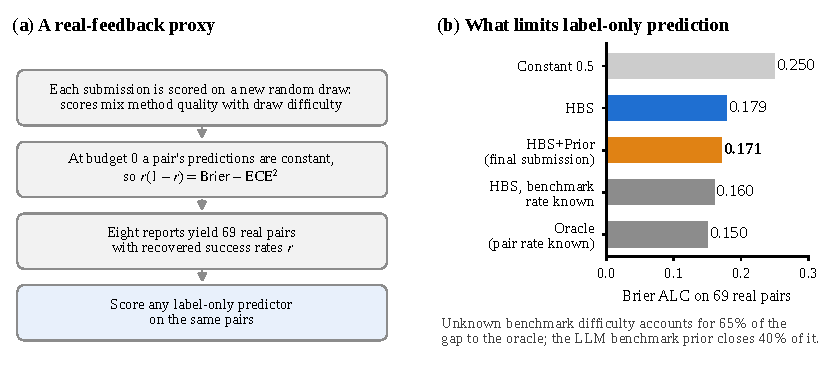
\includegraphics[width=0.8\linewidth]{figures/teaser.pdf}
  \caption{Overview. (a) Recovering each pair's success rate from formative feedback allows all label-only predictors to be scored on the same 69 real pairs. (b) Brier ALC on these pairs. Knowing each benchmark's success rate in advance ($\alpha = 6$) would remove most of the gap between HBS and the oracle; the LLM benchmark prior of our final submission recovers almost half of that improvement.}
  \label{fig:teaser}
\end{figure}

\section{Introduction}
\label{sec:intro}

Evaluating every AI system on every benchmark item is increasingly expensive, particularly for agentic benchmarks, in which a single attempt may involve a long tool-use trajectory. Predictive evaluation reduces this cost by estimating the probability that a system solves an item from attributes of the system and the item and from a few observed outcomes~\citep{truong2025reliable,maiapolo2024tinybenchmarks}. Most existing methods calibrate item parameters on a population of systems that have already been evaluated on the same benchmark.

The Predictive AI Evaluation Competition (PAIEC)~\citep{paiec2026} removes this assumption. Every test item comes from a benchmark absent from the public training pool, a predictor observes at most 31 outcomes per subject--benchmark pair, and predictions are scored by the Brier score averaged over label budgets, an area under the learning curve (Brier ALC). We call this setting \emph{benchmark-level cold start}: before the first label arrives, nothing measured on the test benchmark is available, and afterwards too little is available to calibrate item parameters.

Developing methods for this setting also raises a measurement problem. Formative feedback for each submission is computed on a newly sampled set of pairs, and these samples differ widely in difficulty. Across the eight samples from which we build our proxy, an oracle that knows each pair's success rate scores between 0.099 and 0.183, whereas the methods we wished to compare differ by less than 0.01. Raw scores can therefore rank methods incorrectly. A variant of our method with a subject-ability adjustment scored 0.164 and HBS scored 0.188, yet on identical pairs the variant is worse by 0.026 (Section~\ref{sec:labelonly}).

We make three contributions (Figure~\ref{fig:teaser}):
\begin{enumerate}
  \item \textbf{The bottleneck is the benchmark prior.} More than half of the gap between a strong label-only predictor and an oracle comes from not knowing a new benchmark's difficulty before its labels arrive (Section~\ref{sec:gap}). Item-level difficulty estimates from open LLMs did not transfer to the test benchmarks, but averaged over a benchmark's items, the ratings of a recent open model recover about two fifths of the missing prior on the seven test benchmarks, and almost half once the prior is spread (Sections~\ref{sec:text} and~\ref{sec:prior}).
  \item \textbf{A real-feedback proxy.} When the budget-0 prediction is constant within a pair, the pair's success rate follows from its budget-0 Brier score and expected calibration error (ECE) (Proposition~\ref{prop:identity}). Our eight reports yield 69 pairs on which label-only predictors can be compared, and the proxy reproduces our submissions' scores within label noise (Section~\ref{sec:proxy}).
  \item \textbf{A strong label-only predictor.} Hierarchical Beta-Binomial shrinkage (HBS) pools labels across subjects and benchmarks and needs no training or pretrained model (Section~\ref{sec:method}). On the proxy it outperforms a Bayes-optimal predictor restricted to each pair's own labels, and no label-only variant we tested improves on it by more than 0.0004 (Section~\ref{sec:labelonly}).
\end{enumerate}
Our final submission combines HBS with the LLM benchmark prior (HBS+Prior).\footnote{Codabench submission \finalid. HBS alone, which needs no GPU or pretrained model, is submission 952533.} Code to reproduce all results is available at \url{https://github.com/kay0601/how-far-can-labels-go}.

\section{Related work}
\label{sec:related}

\paragraph{Efficient and predictive evaluation.} Item response theory (IRT)~\citep{lord1980applications} underlies most work on cheaper evaluation: tinyBenchmarks~\citep{maiapolo2024tinybenchmarks} estimate accuracy from about 100 curated items, ATLAS~\citep{li2025atlas} selects items by Fisher information, and \citet{truong2025reliable} predict item difficulty from content. All need item parameters from systems already evaluated on the same benchmark, which benchmark-level cold start lacks.

\paragraph{Extending evaluation to new benchmarks.} \citet{habba2026growing} place new benchmarks on an existing IRT scale using anchor items answered by many models, which one or two subjects per test benchmark cannot provide. Observational scaling laws~\citep{ruan2024observational} and BenchPress~\citep{zeng2026benchpress} predict a model's scores on held-out benchmarks from its other scores. Here, the benchmarks rather than the models are new.

\paragraph{Predicting difficulty from content.} \citet{krsteski2026predicting} predict task difficulty across 17 agentic benchmarks from reasoning-trace entropy, embeddings and metadata. Their leave-one-benchmark-out Spearman correlation of 0.225 is close to our 0.24 to 0.28 (Section~\ref{sec:text}), and they call transfer to unseen benchmarks open. \citet{zhou2025general} annotate 18 demand rubrics per item with GPT-4o and train an assessor for each AI system, reaching an AUROC of 0.747 on held-out benchmarks, but need a proprietary annotator and per-system training data, whereas the test subjects are new. \citet{park2025anticipatory} predict benchmark scores from descriptions of the task and setup.

\paragraph{Shrinkage and probabilistic forecasts.} HBS is an empirical-Bayes estimator~\citep{efron1975data}. Predictions are scored with the Brier score~\citep{brier1950verification} and expected calibration error~\citep{guo2017calibration}, and our proxy uses the single-bin case of Murphy's decomposition~\citep{murphy1973new}.

\paragraph{Concurrent work.} Another PAIEC entry~\citep{aghasalim2026shrunk} uses a shrunk logistic predictor and compares versions by regressing each pair's Brier ALC on its budget-0 Brier score over 42 submissions, whereas our proxy compares methods on identical pairs. It also finds that item-text features and sentence embeddings do not help on new benchmarks.

\section{Problem setup}
\label{sec:setup}

\paragraph{Task.} A \emph{subject} $s$ is an AI system together with its evaluation settings (model, provider, dates, harness, reasoning effort). An \emph{item} $i$ belongs to a benchmark $b(i)$ and is described by its text, structured features (\texttt{item\_features}), interactors and an anonymous benchmark identifier. The outcome $y_{si} \in \{0,1\}$ records whether $s$ solved $i$. A \emph{pair} $j=(s,b)$ is a subject--benchmark combination with at least 80 items, split evenly into acquisition items $A_j$ and evaluation items $E_j$; its \emph{success rate} is $r_j = |E_j|^{-1} \sum_{i \in E_j} y_{si}$. A \emph{draw} $D$ is the set of pairs sampled to score one submission. At label budget $t \in \mathcal{T} = \{0, 1, 3, 7, 15, 31\}$, the outcomes of up to $t$ items from $A_j$ have been revealed for every pair $j \in D$; we write $\mathcal{L}_t$ for all labels revealed in the draw. A predictor $f(s, i; \mathcal{L}_t) \in [0,1]$ is called for every evaluation item at every budget, and every call receives all of $\mathcal{L}_t$. By default, labels are acquired in random order, but a submission may supply its own acquisition policy.

\paragraph{Metric.} At budget $t$, pair $j$ is scored by the Brier score of its evaluation items, and Brier ALC averages a weighted sum over budgets across the pairs of a draw:
\begin{equation}
  \Brier_j(t) = \frac{1}{|E_j|} \sum_{i \in E_j} \bigl(f(s, i; \mathcal{L}_t) - y_{si}\bigr)^2, \qquad
  \ALC(f; D) = \frac{1}{|D|} \sum_{j \in D} \sum_{t \in \mathcal{T}} w_t \, \Brier_j(t),
  \label{eq:alc}
\end{equation}
with $w_0 = w_{31} = 0.1$ and $w_1 = w_3 = w_7 = w_{15} = 0.2$, so that the weights sum to one. Lower is better. For each pair and budget, formative feedback reports $\Brier_j(t)$ and the expected calibration error over ten equal-width bins,
\begin{equation}
  \ECE_j(t) = \sum_{m=1}^{10} \frac{|E_{jm}|}{|E_j|} \, \Bigl| \frac{1}{|E_{jm}|} \sum_{i \in E_{jm}} \bigl(f(s, i; \mathcal{L}_t) - y_{si}\bigr) \Bigr|,
  \label{eq:ece}
\end{equation}
where $E_{jm} \subseteq E_j$ contains the items whose prediction falls in bin $m$.

\paragraph{Data.} Benchmarks were assigned at random to disjoint training and test pools before curation. We use the binary benchmarks of the public training pool of measurement-db~\citep{measurementdb}, four of which have several subjects per item (Table~\ref{tab:data} in Appendix~\ref{app:repro}). Each formative submission is scored on a draw of at most 1,000 subject--item responses. The eight draws from which we build the proxy contain 8 or 9 pairs each, mostly with one subject per benchmark, from seven test benchmarks in total. The final ranking uses a common hidden test subset.

\paragraph{Offline simulator.} Methods that use item text, and those developed before the proxy, are evaluated on 400 draws simulated from the four multi-subject training benchmarks like test draws: about eight pairs per draw, mostly one subject per benchmark, 88 to 230 items per pair and random acquisition. Methods that use item text are selected leave-one-benchmark-out (LOBO).

\section{Hierarchical Beta-Binomial shrinkage}
\label{sec:method}

HBS estimates a success rate for each pair by shrinking every level of a three-level hierarchy (global, benchmark, pair) toward the level above it, and then applies two small item-level corrections. HBS computes every quantity from $\mathcal{L}_t$ within the call and keeps no state between calls. Apart from its hyperparameters, nothing is fitted to training data.

\paragraph{Pair estimate.} For a target pair $(s,b)$, let $k_{sb}$ and $n_{sb}$ be the subject's successes and labels on $b$ in $\mathcal{L}_t$, let $K_{-s,b}$ and $N_{-s,b}$ be those of all other subjects on $b$, and let $K_{-b}$ and $N_{-b}$ be those on all other benchmarks. HBS computes
\begin{equation}
  g_b = \frac{K_{-b} + \kappa_0 \, \mu_0}{N_{-b} + \kappa_0}, \qquad
  \pi_{sb} = \frac{K_{-s,b} + \kappa_1 \, g_b}{N_{-s,b} + \kappa_1}, \qquad
  \bar p_{sb} = \frac{k_{sb} + \alpha \, \pi_{sb}}{n_{sb} + \alpha}.
  \label{eq:hbs}
\end{equation}
Each step is the posterior mean of a Beta-Binomial model whose prior has its mean at the level above and a strength of $\kappa_0$, $\kappa_1$ or $\alpha$ pseudo-labels. The global rate $g_b$ is shrunk strongly toward $\mu_0$ because success rates differ widely across benchmarks, so labels on other benchmarks say little about $b$. The benchmark rate $\pi_{sb}$ excludes the target subject's own labels, which already enter $\bar p_{sb}$ and would otherwise be counted twice. At budget 0, $\mathcal{L}_0$ is empty and HBS predicts $\mu_0$.

\paragraph{Item and group corrections.} Let $R(i)$ be the labels that other subjects received on the same item $i$, and $G(i)$ the labels, from any subject including $s$, on items of the same benchmark that share $i$'s feature group, given by the non-numeric fields of \texttt{item\_features} (Appendix~\ref{app:repro}), which identify, for example, a contest, website, paper or programming language. For a multiset $S$ of labels $(s', i', y)$, let $\Delta(S) = \sum_{(s', i', y) \in S} (y - \bar p_{s' b})$ be the summed residual of each label against the estimate of Equation~\eqref{eq:hbs} for its own pair $(s', b)$. The prediction is
\begin{equation}
  \hat p_{si} = \operatorname{clip}_{[\epsilon,\, 1-\epsilon]} \Bigl( \bar p_{sb}
    + \gamma_I \, \frac{\Delta(R(i))}{|R(i)| + \kappa_I}
    + \gamma_G \, \frac{\Delta(G(i))}{|G(i)| + \kappa_G} \Bigr).
  \label{eq:corrections}
\end{equation}
The item correction needs another subject's label on item $i$; removing it raises the simulated Brier ALC by only 0.0002. The group correction transfers within-benchmark difficulty structure, such as a hard contest, once its labels arrive. Because $G(i)$ includes the target pair's own labels, and labels on item $i$ also enter $R(i)$, the group correction also weakens the shrinkage of $\bar p_{sb}$ when a benchmark's items share one group (Appendix~\ref{app:repro}), and the hyperparameters were tuned with this behavior.

\paragraph{Hyperparameters.} We use $\mu_0 = 0.35$, $\kappa_0 = 100$, $\kappa_1 = \alpha = 3$, $\kappa_I = 1$, $\gamma_I = 1$, $\kappa_G = 5$, $\gamma_G = 0.75$ and $\epsilon = 0.01$ (Table~\ref{tab:hparams} in Appendix~\ref{app:repro}). They were chosen with the offline simulator (Section~\ref{sec:setup}) and the reports of the smoothed mean and HBS+Ability (Appendix~\ref{app:versions}), and re-tuning them on the proxy does not help (Section~\ref{sec:labelonly}). HBS is about 170 lines of plain Python.

\paragraph{LLM benchmark prior (HBS+Prior).} HBS+Prior replaces the constant $\mu_0$ with a benchmark-specific prior estimated from item text. Each item to be predicted is rated by Qwen3.8-27B~\citep{qwen38}, quantized to 4 bits~\citep{dettmers2023qlora}, with an anchored prompt that shows twelve items from the four multi-subject training benchmarks together with their observed success rates (Appendix~\ref{app:prompts}). The rating is $\rho_i = (\mathbb{E}[d] + 0.5)/10$, where $\mathbb{E}[d]$ is the expected digit under the model's next-token distribution over the digits 0 to 9. With $I_b$ the items rated so far on benchmark $b$, the prior
\begin{equation}
  \mu_b = \frac{\sum_{i \in I_b} \rho_i + K_0 \, \mu_0}{|I_b| + K_0}, \qquad K_0 = 5,
  \label{eq:prior}
\end{equation}
replaces $\mu_0$ in the global rate $g_b$ of Equation~\eqref{eq:hbs}. Our final submission also spreads the prior to $\min(0.95, \max(0.05, \mu_0 + 1.5(\mu_b - \mu_0)))$, with $K_0 = 5$, fixes $g_b$ at it ($\kappa_0 \to \infty$), so that labels on other benchmarks do not dilute it, and uses $\alpha = 4$; these settings were chosen on the proxy (Section~\ref{sec:prior}). Unlike HBS, HBS+Prior keeps state. It caches ratings across calls, budgets and subjects, so $\mu_b$ averages all rated items of the benchmark from budget 1 onward and grows item by item at budget 0, where its predictions therefore vary within a pair (Appendix~\ref{app:repro}).

\section{Evaluating methods with formative feedback}
\label{sec:proxy}

To compare methods on the same pairs, we recover the success rate of every pair in our reports and build a proxy on them.

\subsection{Recovering pair success rates}

\begin{proposition}
  \label{prop:identity}
  If the budget-0 prediction is a constant $p_j$ on the evaluation items of pair $j$, then $\Brier_j(0) = r_j(1 - r_j) + (p_j - r_j)^2$ and $\ECE_j(0) = |p_j - r_j|$. Consequently,
  \begin{equation}
    r_j (1 - r_j) = \Brier_j(0) - \ECE_j(0)^2 .
    \label{eq:identity}
  \end{equation}
\end{proposition}

\begin{proof}
  Because $y_{si}^2 = y_{si}$, $\Brier_j(0) = |E_j|^{-1} \sum_{i \in E_j} (p_j^2 - 2 p_j y_{si} + y_{si}) = p_j^2 - 2 p_j r_j + r_j = r_j(1 - r_j) + (p_j - r_j)^2$. All predictions fall into the same bin, so Equation~\eqref{eq:ece} reduces to $|p_j - r_j|$.
\end{proof}

The condition holds for HBS, and for any predictor whose budget-0 output depends only on the subject and the benchmark, because no labels are available at budget 0. Equation~\eqref{eq:identity} determines $r_j$ up to the reflection $r_j \leftrightarrow 1 - r_j$. When $p_j \neq 1/2$ is known, $\Brier_j(0) = p_j^2 + (1 - 2p_j)\, r_j$ gives $r_j$ directly. The prediction is unknown for 43 pairs: 34 from four early submissions whose code we did not retain, and 9 from HBS+Ability, whose prediction is constant within a pair but depends on subject metadata that the logs anonymize. For these, we choose the root closer to the rates of the same benchmark in the reports whose prediction is known. On the 26 pairs with known roots, from the reports of the smoothed mean, HBS and HBS+ItemLLM, the rule is correct for 25 (Appendix~\ref{app:robust}).

\paragraph{Oracle limit of a draw.} A predictor that knows every $r_j$ and predicts it at every budget scores $\Brier_j(t) = r_j(1 - r_j)$, so by Equation~\eqref{eq:alc} its Brier ALC is
\begin{equation}
  \bar v(D) = \frac{1}{|D|} \sum_{j \in D} r_j (1 - r_j).
\end{equation}
By Proposition~\ref{prop:identity}, no predictor that is constant within each pair can score below $\bar v(D)$. We call $\bar v(D)$ the \emph{oracle limit} of the draw. Across our eight reports it ranges from 0.099 to 0.183 (Figure~\ref{fig:draws} in Appendix~\ref{app:versions}), and the two best raw scores were obtained on the two easiest draws.

\subsection{The proxy}

The proxy scores a label-only predictor $f$ on the 69 recovered pairs. For each report, we draw label sequences $y_{j1}, \dots, y_{j31} \sim \mathrm{Bernoulli}(r_j)$ independently for its pairs, reveal the first $t$ labels of every pair at budget $t$, and query $f$ with item inputs that carry only the subject and the benchmark identifier. Since the outcomes on $E_j$ average to $r_j$, the Brier score of a prediction $p_j(t)$ is exactly $r_j(1 - r_j) + (p_j(t) - r_j)^2$, and averaging over label sequences gives $f$'s expected Brier ALC on the report. The pairs of a report are simulated jointly, so pooling behaves as on the real draw. Parameters are selected leave-one-report-out, and 95\% intervals come from resampling whole reports.

\paragraph{Validity.} For the three submissions whose code we retained (the smoothed mean, HBS+Ability and HBS; Appendix~\ref{app:versions}), Table~\ref{tab:proxy} compares the real score with the proxy's expectation for the same predictor on the same pairs, and with the spread due to label noise. Every real score lies 0.006 to 0.010 below its expectation, within 1.3 standard deviations. The item and group corrections, which the proxy disables, account for about 0.0015 of this difference, and the rest is consistent with favorable label sequences (Appendix~\ref{app:robust}). At the pair level, 24 of the 25 pairs with label noise lie within two standard deviations. We therefore use it as our primary criterion for label-only predictors.

\begin{table}[t]
  \caption{Real Brier ALC and the proxy's expectation for the same predictor and pairs; SD is the spread due to label noise alone, and differences are computed before rounding. HBS+Ability's rates are inferred (Section~\ref{sec:proxy}).}
  \label{tab:proxy}
  \centering
  \small
  \begin{tabular}{lrrrrr}
    \toprule
    Submission & Real & Proxy & SD & Real $-$ proxy & $z$ \\
    \midrule
    Smoothed mean & 0.1829 & 0.1899 & 0.0069 & $-0.0070$ & $-1.0$ \\
    HBS+Ability & 0.1639 & 0.1741 & 0.0076 & $-0.0103$ & $-1.3$ \\
    HBS & 0.1883 & 0.1946 & 0.0077 & $-0.0063$ & $-0.8$ \\
    \bottomrule
  \end{tabular}
\end{table}

\subsection{Measuring an LLM prior on the test benchmarks}
\label{sec:measure}

The proof of Proposition~\ref{prop:identity} applies at any budget at which predictions are constant within each pair, in which case $\ECE_j(t) = |p_j(t) - r_j|$. We used this in one measurement submission, not intended as a final entry, to estimate the LLM prior of Equation~\eqref{eq:prior} on the test benchmarks. At budget 0 it rated and cached every item but predicted the constant 0.35, which identifies $r_j$ and fixes $\mu_b$ from budget 1. At budget 1 it predicted the prior $\mu_b$, which yields $|\mu_b - r_j|$ but not its sign, and at budget 3 it predicted $\mu_b + 0.1$, which breaks this symmetry. In simulation, this procedure recovers $\mu_b$ exactly, and in the real run every pair's budget-1 scores fit a constant prediction. Because benchmark identifiers are fixed across submissions, the proxy can then score HBS+Prior on all 69 pairs.

\paragraph{Use of formative feedback.} The proxy and the measurement submission rely only on our own formative feedback, which the competition provides to guide development. We used the recovered rates and priors only to compare methods offline. No recovered value is written into any submitted program, we made no attempt to identify the subjects or benchmarks behind the anonymous identifiers, and we do not release these values.

\section{Experiments}
\label{sec:experiments}

\subsection{Label-only prediction}
\label{sec:labelonly}

On the 69 proxy pairs, HBS scores 0.179, compared with 0.207 for the organizers' empirical-mean baseline, 0.250 for a constant prediction of 0.5 and 0.150 for the oracle (Table~\ref{tab:labelonly}). Pooling the labels of other subjects on the same benchmark matters. Removing it costs 0.0030, as much as replacing HBS with the simpler smoothed mean (0.0028), although pooling changes predictions only for the 26 pairs that share their benchmark with another subject in the same draw. A Bayes-optimal predictor that knows the distribution of the other pairs' success rates but sees only the target pair's labels is worse than HBS by 0.0024, although estimating that distribution on the same reports favors it. Neither a mixture prior with a near-zero component nor re-tuning $\mu_0$, $\alpha$ and $\kappa_1$ on held-out reports improves on HBS, and stratified label acquisition gains only 0.0004 in simulation. These conclusions also hold on the six reports that did not inform the design of HBS and on the 26 pairs whose root is known, where the differences to the baseline, the smoothed mean, HBS without pooling and the own-label predictor are $+0.024$, $+0.005$, $+0.005$ and $+0.003$ (Appendix~\ref{app:robust}).

\paragraph{Subject-ability adjustment.} HBS+Ability shifts the benchmark prior in logit space by a subject ability fitted on training data (Appendix~\ref{app:versions}). It helped in simulation, but on real feedback it raised the budget-0 Brier score to 0.326, worse than predicting 0.5, and lost 0.026 to HBS on its draw. The training pool holds many older systems; the test subjects are recent ones on harder benchmarks.

\begin{table}[t]
  \caption{Label-only alternatives to HBS. Positive changes in Brier ALC are worse; intervals are 95\% intervals from resampling whole reports with the inferred roots held fixed, and for the single-draw HBS+Ability row, SD is that of the paired difference. HBS scores 0.179 on the proxy.}
  \label{tab:labelonly}
  \centering
  \small
  \begin{tabular}{>{\raggedright\arraybackslash}p{0.40\linewidth}>{\raggedright\arraybackslash}p{0.19\linewidth}>{\raggedright\arraybackslash}p{0.31\linewidth}}
    \toprule
    Alternative to HBS & Selection & Change in Brier ALC \\
    \midrule
    \multicolumn{3}{l}{\emph{Real-feedback proxy, 69 pairs}} \\
    Official empirical-mean baseline & reference & $+0.0282$ $[+0.0234, +0.0324]$ \\
    Smoothed mean & fixed & $+0.0028$ $[+0.0013, +0.0043]$ \\
    Benchmark pooling removed ($\kappa_1 \to \infty$) & fixed & $+0.0030$ $[+0.0015, +0.0045]$ \\
    Bayes-optimal own-label predictor & reference & $+0.0024$ $[+0.0014, +0.0034]$ \\
    Mixture prior with a near-zero component & leave-one-report-out & $+0.0004$ $[-0.0004, +0.0008]$ \\
    Re-tuned $\mu_0$, $\alpha$, $\kappa_1$ & leave-one-report-out & $+0.0006$ $[-0.0008, +0.0015]$ \\
    HBS+Ability, on its own draw & fixed & $+0.0265$ (SD 0.0045) \\
    \midrule
    \multicolumn{3}{l}{\emph{Offline simulator, 400 draws}} \\
    Stratified label acquisition & fixed & $-0.0004$ (SE 0.0001) \\
    Group correction removed & fixed & $+0.0011$ (SE 0.0001) \\
    \bottomrule
  \end{tabular}
\end{table}

\subsection{Where the remaining error lies}
\label{sec:gap}

On the 69 pairs, HBS is 0.029 above the oracle. To locate this gap, we gave HBS each benchmark's mean success rate in advance, estimated from the other reports, in place of $\mu_0$. With the pair-prior strength of HBS ($\alpha = 3$), this lowers its score to 0.162 and closes 58\% of the gap (95\% interval 54 to 61\%). With $\alpha = 6$, which suits an accurate prior, it closes 65\% (60 to 69\%). On the 26 pairs with known roots, $\alpha = 3$ and $\alpha = 6$ close 54\% and 56\%. The loss is concentrated at budgets 0 to 3, where HBS relies on its global prior, and vanishes by budget 31 (Figure~\ref{fig:gap}). The remainder reflects differences between subjects on the same benchmark and the error in each benchmark's estimated rate. This diagnostic uses rates recovered from test feedback and could not be part of a submission.

\begin{figure}[t]
  \centering
  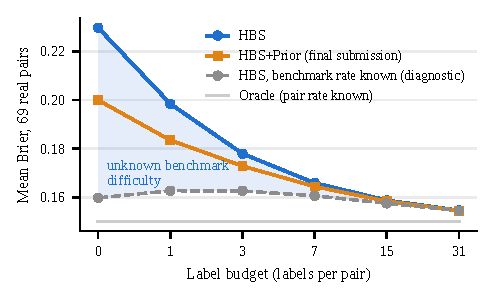
\includegraphics[width=0.46\linewidth]{figures/gap_by_budget.pdf}
  \caption{Mean Brier per budget on the 69 real pairs. Knowing each benchmark's rate ($\alpha = 6$; ALC 0.162 with $\alpha = 3$) removes most of HBS's low-budget error, and the LLM prior part of it.}
  \label{fig:gap}
\end{figure}

\subsection{Can item text close the gap?}
\label{sec:text}

Before any labels arrive, item text is the only information available about a new benchmark. We evaluated open LLMs that fit on the competition's hardware, holding out one of the four multi-subject training benchmarks at a time and using each item's success rate averaged over subjects as the target (prompts in Appendix~\ref{app:prompts}; further details in Appendices~\ref{app:repro} and~\ref{app:llm}).

\paragraph{Item difficulty within a benchmark.} We prompted Qwen3-8B and Qwen3-32B~\citep{yang2025qwen3} to rate 5,322 training items and fitted a ridge-regression probe on the last prompt token's hidden state. On the held-out benchmark, the probe ranks items with an average Spearman correlation of 0.24 (8B) and 0.28 (32B), compared with $-0.03$ for bge-small sentence embeddings~\citep{xiao2024cpack}. In the simulator, the probe scores improved Brier ALC by 0.003 (8B) and 0.005 (32B).

\paragraph{Benchmark difficulty.} Without examples, both Qwen3 models rated every training benchmark between 6.8 and 7.7 out of 9 on average, although the benchmarks' mean success rates over all items range from 0.22 to 0.62. With nine anchor items from the other benchmarks and their observed success rates in the prompt, only Qwen3.8-27B, the most recent of the four models, produced a benchmark-level prior better than the constant of HBS (budget-0 Brier score 0.217 against 0.233). Qwen3-8B, Qwen3.5-9B~\citep{qwen35} and the larger but older Qwen3-32B did not (Table~\ref{tab:bench} in Appendix~\ref{app:llm}), and only Qwen3.8-27B was later measured on the test benchmarks. A single rating is noisy, but a predictor can average its ratings over a benchmark's items. Four training benchmarks are too few to validate this, so we evaluated it on the test benchmarks (Section~\ref{sec:prior}).

\paragraph{Item-level shift on real feedback.}
\label{sec:itemllm}
To test the item-level signal on real data, we submitted HBS+ItemLLM, which shifts the HBS estimate in logit space by $\gamma(z_i - c)$, where $z_i$ is the item's standardized Qwen3-32B probe score, $c$ is the mean score of the target and the labeled items of its benchmark, and $\gamma = 0.5$. It improved the simulator by 0.005, with $\gamma$ selected leave-one-benchmark-out, and ran as intended, yet it scored 0.157 on its real draw, where the proxy expects 0.131 for HBS (3.8 standard deviations of label noise). The loss falls from 0.070 at budget 1 to 0.024 at budget 7 and is near zero from budget 15 (Figure~\ref{fig:text}b in Appendix~\ref{app:llm}). About 70\% of it comes from the two pairs of one benchmark, whose shifts are centered on the same labeled items, which points to a cause on that benchmark, such as extreme scores among its first revealed items. Training-like scores leave HBS nearly unchanged, and the feedback cannot identify the cause (Appendix~\ref{app:llm}).

\subsection{A benchmark prior from an LLM}
\label{sec:prior}

The measurement submission (Section~\ref{sec:measure}) recovered the prior of all seven test benchmarks. The priors order the benchmarks' mean success rates across our reports with Kendall's $\tau = 0.62$ and are closer to them than the constant 0.35 for five of the seven, but they are compressed toward the middle (Appendix~\ref{app:robust}). Used from budget 1, the prior improves on HBS by 0.004. Used from budget 0, where it accumulates item by item, it improves on HBS by 0.007 (95\% interval 0.006 to 0.009; Table~\ref{tab:prior} in Appendix~\ref{app:robust}), mostly at budgets 0 to 3 (Figure~\ref{fig:gap}). This is 44\% of what knowing each benchmark's rate gains at the same $\alpha$, and 39\% with $\alpha = 6$. On the 26 pairs with known roots, it is 0.008 and holds in each of their three reports. Removing any one benchmark leaves 0.006 to 0.009, but treated as a sample of benchmarks, the seven give a jackknife standard error of 0.0033, so an approximate 95\% interval for the change in Brier ALC on new benchmarks reaches from $-0.015$ to $+0.001$.

\paragraph{Settings of the final submission.} Because the priors are compressed, we searched on the proxy over the factor by which the prior is spread around $\mu_0$ (1 to 2), $\alpha$ (2 to 8), $\kappa_0$ (100 or $\infty$) and $K_0$ (0 to 5). Chosen leave-one-report-out, the same setting wins in every fold: a factor of 1.5, $\alpha = 4$ and $\kappa_0 \to \infty$, which add 0.0017 (95\% interval 0.0008 to 0.0026). The final submission thus improves on HBS by 0.009 (0.007 to 0.011), 48\% of the diagnostic's gain. Chosen leave-one-benchmark-out, which tests new benchmarks, the spread factor varies from 1.25 to 2, and the held-out benchmarks lose 0.0012 against the unspread prior; the jackknife standard error rises to 0.0048 (Appendix~\ref{app:robust}).

Formative runs on fresh draws match the proxy within label noise (Table~\ref{tab:final_run} in Appendix~\ref{app:robust}): the settings of HBS scored 0.174 (expected 0.180 for HBS, 0.171 for them), the final submission 0.151 (0.168 and 0.159).

\section{Discussion and limitations}
\label{sec:discussion}

\paragraph{Benchmark-level cold start is limited by information.} How difficult a benchmark is for current systems depends on grading strictness, the harness and environment, and recent progress in model capabilities, none of which is stated in its items. Success rates in the test pool cluster by benchmark, so the first few labels are highly informative, whereas a text-based prior helps only if it reflects current capabilities. In our experiments, LLMs judged a task type's difficulty better than an item's.

\paragraph{Simulation can mislead.} Two changes that helped on the public training pool hurt on real feedback, and both relied on statistics learned across that pool. The subject-ability adjustment assumed its older population of systems, and the item-level shift assumed that difficulty signals from four benchmarks transfer. Leave-one-benchmark-out validation on so few benchmarks cannot detect such shifts, so we adopted changes only if they held on real feedback.

\paragraph{Limitations.} The proxy omits item and group structure, treats labels as independent Bernoulli draws, is pessimistic by 0.006 to 0.010 (Table~\ref{tab:proxy}) and cannot evaluate text-based methods. Its intervals hold the seven benchmarks and the 43 inferred roots fixed; the comparisons with HBS without pooling and the own-label predictor, and the share due to benchmark difficulty, survive the estimated root errors but not uniform flips at the rule's upper error bound (Appendix~\ref{app:robust}). The 69 pairs come from seven test benchmarks, and the hidden final test subset may differ. The verdict on the item-level shift rests on one real draw, although five of its nine pairs lost. The LLM prior was measured once, on the seven test benchmarks, where its final settings were also chosen, and without a GPU the final submission falls back to HBS. We tested only open models of at most 32B parameters.

\section{Conclusion}

In benchmark-level cold start, the main limitation is missing information about the new benchmark, not the predictor. No label-only alternative we tested improves on hierarchical shrinkage by more than 0.0004, and more than half of its remaining error comes from not knowing an unseen benchmark's difficulty. On the seven test benchmarks, averaging a recent open LLM's ratings over a benchmark's items supplies almost half of this missing prior, but its value for new benchmarks is uncertain. A reliable judge of benchmark difficulty would be worth up to 0.019 Brier ALC here.

\begin{ack}
This study was supported in part by the National Science and Technology Council (NSTC), Taiwan, under grants 115-2627-M-006-001, 115-2218-E-A49-023, and 115-2634-F-A49-014. We thank the National Center for High-performance Computing (NCHC) of the National Applied Research Laboratories (NARLabs) in Taiwan for providing computational and storage resources. The authors declare no competing interests.
\end{ack}

\bibliographystyle{plainnat}
\bibliography{references}

\clearpage
\appendix

\section{Submissions}
\label{app:versions}

Table~\ref{tab:versions} lists the formative submissions referred to in this paper. In Figure~\ref{fig:draws}, \emph{Early 1} to \emph{Early 4} denote the four early submissions in the order listed. Their predictors are not evaluated in this paper, but their feedback reports contribute 34 pairs to the proxy.

\begin{table}[ht]
  \caption{Formative submissions and their Codabench identifiers.}
  \label{tab:versions}
  \centering
  \small
  \begin{tabular}{l>{\raggedright\arraybackslash}p{0.52\linewidth}>{\raggedright\arraybackslash}p{0.21\linewidth}}
    \toprule
    Method & Description & Codabench ID \\
    \midrule
    Early submissions & Our first predictors, made before the methods in this paper; code not retained & 928061, 930136, 930165, 931142 \\
    Smoothed mean & Pair's label mean shrunk ($\alpha = 5$) toward the benchmark's label mean, itself shrunk toward 0.35 with strength 30; with the item correction & 951748 \\
    HBS+Ability & HBS with a prior mean of 0.4 and a subject-ability shift estimated on the training data & 951853 \\
    HBS & Section~\ref{sec:method}; label-only & 952533 \\
    HBS+ItemLLM & HBS with an item-level shift from Qwen3-32B representations (Section~\ref{sec:itemllm}) & 960385 \\
    Measurement & Measures the LLM benchmark prior on the test benchmarks (Section~\ref{sec:measure}); not a candidate for the final ranking & 978024 \\
    HBS+Prior & HBS with the LLM benchmark prior from budget 0 (Section~\ref{sec:method}), settings of HBS; formative run in Table~\ref{tab:final_run} & 978186 \\
    HBS+Prior & The same with the settings of Section~\ref{sec:prior}; final submission & \finalid \\
    \bottomrule
  \end{tabular}
\end{table}

\paragraph{Smoothed mean.} With $k_b$ and $n_b$ the successes and labels of all subjects on benchmark $b$, including the target subject, the pair estimate is $(k_{sb} + 5 m_b)/(n_{sb} + 5)$ with $m_b = (k_b + 30 \cdot 0.35)/(n_b + 30)$. It adds the item correction of Equation~\eqref{eq:corrections} with $\kappa_I = \gamma_I = 1$, where residuals are taken against the same pair estimates, and clips to $[0.01, 0.99]$; it has no group correction.

\paragraph{HBS+Ability.} It uses Equation~\eqref{eq:hbs} with $\mu_0 = 0.4$ and moves $\pi_{sb}$, clipped to $[0.01, 0.99]$, by $\beta a_s$ in logit space before the pair update, with $\beta = 0.55$. The ability $a_s$ comes from the training pairs with at least 80 items, fitted by alternating least squares in $\operatorname{logit}(r_{sb}) = d_b + a_s$ with rates clipped to $[0.01, 0.99]$ and abilities centered. A test subject whose model name, or the source model name in its extra features, was seen in training receives that model's ability; otherwise, $a_s$ is predicted by a ridge regression (strength 1, unpenalized intercept) on the centered release year and the reasoning effort on an ordinal scale from 0 to 5 (minimal, low, medium, high, xhigh, max), each with an indicator for a missing value; the release year is the release date as a fractional year, centered on the training mean.

\begin{figure}[ht]
  \centering
  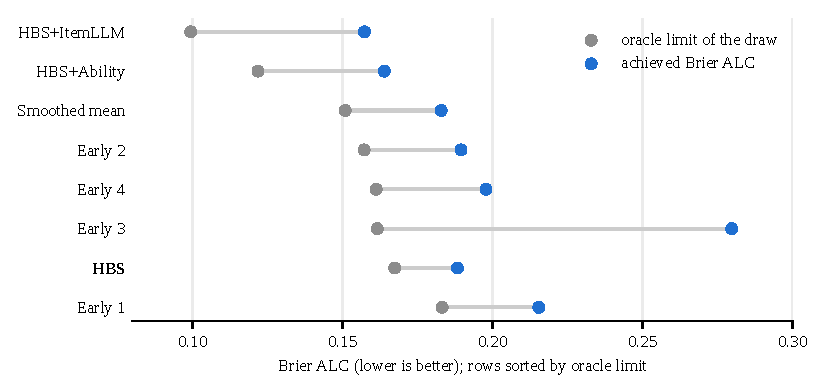
\includegraphics[width=0.655\linewidth]{figures/draw_limits.pdf}
  \caption{Oracle limit and achieved Brier ALC of the eight formative submissions used to build the proxy. The oracle limit measures the difficulty of each draw, independently of the method.}
  \label{fig:draws}
\end{figure}

\section{Prompts}
\label{app:prompts}

All prompts were formatted with the model's chat template, with thinking disabled, followed by the prefilled answer prefix ``\texttt{Rating:\textvisiblespace}'', so that the next token is the rating. We read the probabilities of the digit tokens 0 to 9 at that position and renormalize them. The rating is the expected digit $\mathbb{E}[d]$; for the anchored prompt, it is mapped to a success rate $(\mathbb{E}[d] + 0.5)/10$. The item-difficulty probe uses the hidden states of the zero-shot prompt rather than its rating. \texttt{\{content\}} denotes the item text. A text longer than its limit $L$ keeps its first $h$ tokens and a window of $L - h$ further tokens, joined by ``[\ldots]'' ($h$ = 384 of 2,048 tokens for zero-shot ratings, 64 of 256 for anchors and 192 of 1,024 for targets). The window is the end of the text, unless a \texttt{TODO} marker starts before it (the first occurrence of \texttt{TODO: Implement block}, or else of \texttt{TODO}, which marks the code to write in code-completion items). Then, with the marker at token $m$ and $a = \min(512, \lfloor (L - h)/3 \rfloor)$, the window starts at $\max(h, m + a - (L - h))$, so it ends $a$ tokens after the marker unless that would overlap the head. Token positions are counted with each model's own tokenizer on the item text before it is inserted into the prompt.

\paragraph{Zero-shot rating (item difficulty).} Item texts were truncated to 2,048 tokens.
\begin{promptbox}
Below is a task from an AI evaluation benchmark. A capable AI system (a frontier language model, possibly acting as an agent with tools) will attempt it, and the attempt is graded pass/fail.

\texttt{<task>}\\
\texttt{\{content\}}\\
\texttt{</task>}

Do not attempt the task yourself. How likely is a strong AI system to solve this task correctly? Answer with a single digit from 0 to 9, where 0 means it almost certainly fails and 9 means it almost certainly succeeds.
\end{promptbox}

\paragraph{Anchored rating (benchmark difficulty).} The introduction is followed by the examples in a fixed random order and then by the question: nine examples from the other three benchmarks in the experiments of Section~\ref{sec:text}, and twelve from all four benchmarks in HBS+Prior, a prompt that therefore cannot be evaluated leave-one-benchmark-out on the training benchmarks. The anchors of a benchmark are the items at positions $\lfloor q(N - 1) \rfloor$, $q \in \{0.2, 0.5, 0.8\}$, among its $N$ items with at least five subjects sorted by success rate and then by item identifier, so the 20th, 50th and 80th percentiles; the examples appear in an order shuffled once with seed 0. \texttt{\{pct\}} is the success rate as a rounded percentage, and \texttt{\{digit\}} is $\min(9, \lfloor 10 \times \text{rate} \rfloor)$ of the unrounded rate. In Section~\ref{sec:text}, the targets are 120 random items per benchmark with at least three subjects (seed 0); HBS+Prior rates every item it is asked about.
\begin{promptbox}
You will estimate how often AI systems succeed on a task from an AI evaluation benchmark. The AI systems are language models, often acting as agents with tools, and each attempt is graded pass/fail.

For reference, here are tasks from other benchmarks with the share of AI systems that solved them. A digit d means d*10\% to (d+1)*10\%.

\texttt{<example>}\\
\texttt{<task>}\\
\texttt{\{content\}}\\
\texttt{</task>}\\
Share of AI systems that solved it: \texttt{\{pct\}}\% (digit \texttt{\{digit\}})\\
\texttt{</example>}

[\ldots{} eight further examples (eleven in HBS+Prior) \ldots]

Now a new task, from a different benchmark:

\texttt{<task>}\\
\texttt{\{content\}}\\
\texttt{</task>}

Do not attempt the task yourself. What share of AI systems solve this task? Answer with a single digit from 0 to 9 as defined above.
\end{promptbox}

\section{Reproducibility and implementation details}
\label{app:repro}

\paragraph{Code and data.} Code is available at \url{https://github.com/kay0601/how-far-can-labels-go}; its README lists the command that produces each table and figure. The training data are revision bc8204d of measurement-db, obtained with the official preparation script; \bench{matharena}, which that script excludes, is downloaded separately at the same revision. Formative feedback is private to each team and is not released; the proxy scripts read a team's own scoring logs. The official preparation script excludes \bench{matharena} because about 60 of its responses are not binary; we drop those responses and keep the rest. \bench{mmdocrag} is not used because its scores are continuous, and \bench{swe\_rebench}, with one subject per item, is used for training only.

\paragraph{Feature groups.} \texttt{item\_features} is a list of \texttt{key=value} fields separated by semicolons. The group of an item is its benchmark together with the sorted list of its fields whose value is not a number, except \texttt{prompt\_source}; a value counts as a number if it consists of digits with at most one decimal point. An item without such fields has no group and no group correction. Labels on item $i$ itself from other subjects enter both $R(i)$ and $G(i)$. For a single subject on a benchmark whose items share one group, Equation~\eqref{eq:corrections} turns $\bar p_{sb}$ into the shrinkage estimate $(k_{sb} + \alpha' \pi_{sb})/(n_{sb} + \alpha')$ with $\alpha' = \alpha\, (n_{sb}(1 - \gamma_G) + \kappa_G)/(n_{sb} + \kappa_G + \alpha \gamma_G)$, which is 1.9, 1.7, 1.4, 1.2 and 1.0 at 1, 3, 7, 15 and 31 labels instead of $\alpha = 3$.

\paragraph{Simulator.} Each simulated draw adds pairs until it holds 1,000 items: a random training benchmark and subject, with 88 to 230 of its items chosen uniformly at random. With probability 0.15, a second subject of the same benchmark joins the pair's items if it shares at least 80 of them. Stratified acquisition replays the platform's stream of candidate items: a candidate is revealed if its feature group has no more labels from the pair than the least sampled group so far, or if every remaining candidate is needed to fill the budget; items without a group are always revealed.

\paragraph{HBS+Prior.} The platform calls the predictor sequentially in one worker process and restarts it at each budget, so ratings are written to disk as they are made and reloaded after each restart; each item is rated only once. Only items to be predicted are rated, never revealed acquisition items, and the target item is rated before its prior is computed, so the $k$-th distinct item of a benchmark at budget 0 sees $|I_b| = k$. Each benchmark's sum and count of ratings are shared by all subjects on it, so at budget 0 the prior used for an item depends on how many items of its benchmark, including other subjects' items, were rated before it. The platform calls the predictor once per evaluation item and does not reveal the remaining items, so the prior cannot be computed over all items before the first prediction. Rating one item takes about 3 seconds on an RTX 3090, well within the platform's limit of 120 seconds per call; the 4-bit model needs about 18 GB of GPU memory and is downloaded by the platform from the model list of the submission. If the model cannot be loaded, the submission falls back to HBS.

\paragraph{LLM experiments.} The ridge probe of Section~\ref{sec:text} uses the hidden state of the last prompt token at half, three quarters or all of the model's depth, or the mean over tokens at half depth, with a regularization strength of $10^3$ or $10^4$. The best setting is $10^4$ with layer 27 of 36 for Qwen3-8B and with the final layer, 64, for Qwen3-32B. Qwen3-32B and Qwen3.8-27B were loaded in 4-bit precision (bitsandbytes NF4 with double quantization and bfloat16 computation), and Qwen3-8B and Qwen3.5-9B in bfloat16. The 5,322 rated items are all items of the four multi-subject training benchmarks and 1,000 random items of \bench{swe\_rebench} (seed 0). For HBS+ItemLLM, $z_i$ is the probe's prediction divided by the standard deviation of its leave-one-benchmark-out predictions on the training items.

\begin{table}[ht]
  \caption{Public training benchmarks (measurement-db, revision bc8204d). Only benchmarks with several subjects per item can be used to evaluate methods offline.}
  \label{tab:data}
  \centering
  \small
  \begin{tabular}{lrrl}
    \toprule
    Benchmark & Items & Subjects per item (median) & Use \\
    \midrule
    \bench{multi\_swebench}    & 2,126 & 27 & training and offline evaluation \\
    \bench{matharena}          & 1,751 &  9 & training and offline evaluation \\
    \bench{real\_webagents}    &   233 & 12 & training and offline evaluation \\
    \bench{researchcodebench}  &   212 & 31 & training and offline evaluation \\
    \bench{swe\_rebench}       & 6,306 &  1 & training only \\
    \bottomrule
  \end{tabular}
\end{table}

\begin{table}[ht]
  \caption{Hyperparameters of HBS, with their names in the released code.}
  \label{tab:hparams}
  \centering
  \small
  \begin{tabular}{lllr}
    \toprule
    Symbol & Code name & Role & Value \\
    \midrule
    $\mu_0$ & \texttt{PRIOR\_MEAN} & mean of the global prior & 0.35 \\
    $\kappa_0$ & \texttt{GLOBAL\_K} & strength of the global prior & 100 \\
    $\kappa_1$ & \texttt{BENCH\_K} & strength of the benchmark prior & 3 \\
    $\alpha$ & \texttt{ALPHA} & strength of the pair prior & 3 \\
    $\kappa_I$, $\gamma_I$ & \texttt{ITEM\_K}, \texttt{ITEM\_GAMMA} & shrinkage and scale of the item correction & 1, 1 \\
    $\kappa_G$, $\gamma_G$ & \texttt{GROUP\_K}, \texttt{GROUP\_GAMMA} & shrinkage and scale of the group correction & 5, 0.75 \\
    $\epsilon$ & \texttt{CLIP} & clipping margin & 0.01 \\
    \bottomrule
  \end{tabular}
\end{table}

\paragraph{Compute.} One simulator configuration (400 draws) takes about 10 seconds on a CPU. The LLM experiments ran on a single RTX 3090 (24 GB): extracting Qwen3-8B representations for 5,322 items took 12 minutes and Qwen3-32B representations about 50 minutes; the anchored ratings took 10 minutes for Qwen3.5-9B, 22 minutes for Qwen3-32B and 28 minutes for Qwen3.8-27B. The formative run of the measurement submission, with 491 evaluation items, completed in under 40 minutes. Software: Python 3.13 for HBS and the simulator; Python 3.10 with PyTorch 2.7.1, Transformers 5.2.0 and bitsandbytes 0.50.2 for the LLM experiments.

\section{Disclosures}
\label{app:disclosure}

\begin{itemize}
  \item Training data: only the public training pool of measurement-db (CC BY-SA 4.0, gated access under its terms of use), as listed in Table~\ref{tab:data}. We do not redistribute the data. No external data and no contributions from other teams were used.
  \item Pretrained models: BAAI/bge-small-en-v1.5 (MIT license) and Qwen/Qwen3-8B, Qwen/Qwen3-32B, Qwen/Qwen3.5-9B and Qwen/Qwen3.8-27B (Apache 2.0). The final submission (HBS+Prior) loads Qwen3.8-27B at run time; HBS uses no pretrained model; HBS+ItemLLM loaded Qwen3-32B.
  \item Coding assistant: we used Claude Code (Anthropic) for implementation, analysis and drafting this report.
  \item Broader impact: predictive evaluation can reduce the compute spent on evaluating AI systems. Its main risk is that predicted success rates are trusted in place of measured ones; our results show that predictions are least reliable on unseen benchmarks before labels arrive, which is where such trust would be most tempting. Scores on small random samples also mix the quality of a method with the difficulty of the sample, which matters for anyone who ranks methods on such samples; reporting each draw's oracle limit next to its score, which any team can compute from its own feedback, would separate the two.
\end{itemize}

\FloatBarrier
\section{Robustness of the proxy}
\label{app:robust}

\paragraph{Subsets.} The 26 pairs with known roots come from the reports of the smoothed mean, HBS and HBS+ItemLLM, which predict 0.35 at budget 0. The 26 pairs of Table~\ref{tab:proxy} and Figure~\ref{fig:pairs}, a different set, come from the reports of the three submissions whose code we retained, the smoothed mean, HBS+Ability and HBS; for HBS+Ability, the proxy uses the inferred budget-0 predictions, through an ability table that reproduces them. HBS+ItemLLM predicts 0.35 at budget 0 because its shift vanishes without labels ($c = z_i$). For HBS+Ability, both the root and the sign of $p_j - r_j$ are inferred: for seven of its nine pairs only one sign gives a prediction in $[0, 1]$, and for the other two we take the higher candidate, which differs from the lower one by 0.08 and 0.03. For all three submissions of Table~\ref{tab:proxy}, the budget-0 scores match the proxy by construction, so the table tests budgets 1 to 31. The reference of an inferred pair is the mean rate of its benchmark over the 26 known pairs; the roots of HBS+Ability are inferred first, and for the four early reports the reference also includes its pairs. Every test benchmark appears in all eight reports and contributes 8 to 11 of the 69 pairs and 3 to 5 of the 26 known; 26 of the 69 pairs, 10 of the 26 known, share their benchmark with another subject in the same draw.

\paragraph{Pair-level validity.} Figure~\ref{fig:pairs} compares each pair's real Brier ALC with the proxy's expectation for the three submissions of Table~\ref{tab:proxy}, as a $z$-score under label noise alone. Of the 25 pairs with label noise, 24 lie within two standard deviations, and the mean $z$ of $-0.35$ reflects the proxy's pessimism. The exception ($z = 3.6$, on the draw of HBS) is a pair whose real Brier score rose from 0.27 at budget 0 to 0.34 at budgets 3 to 15. This is consistent with an acquisition half whose success rate differs from that of the evaluation half, which the proxy does not model because it draws labels from the evaluation rate. The one pair without label noise, whose rate is 0 or 1 so that every simulated label sequence is the same, matches its expectation to within $10^{-6}$.

\paragraph{Pessimism of the proxy.} The real scores of Table~\ref{tab:proxy} fall 0.006 to 0.010 below the proxy. The item and group corrections, which the proxy disables, are together worth 0.0015 in the simulator, the group correction alone 0.0011 (Table~\ref{tab:labelonly}). The finite pools of items do not explain the rest. Drawing each pair's labels without replacement from a pool of $|A_j| = |E_j|$ items at exactly the evaluation rate $r_j$ lowers the proxy's expectation by 0.0008 to 0.0009, but under a random split of a pair's items the acquisition half's rate itself varies around $r_j$. Drawing it given $r_j$, with a uniform prior on the pair's underlying rate (the acquisition rate from $\mathrm{Beta}(k_j + 1, |E_j| - k_j + 1)$, with $k_j = r_j|E_j|$ the evaluation successes, then $|A_j| = |E_j|$ items drawn at that rate and revealed without replacement), instead raises the expectation by 0.0022 to 0.0030, and the real scores then lie 1.0 to 1.5 standard deviations below it. In either model, the remaining difference is consistent with favorable label sequences on the three draws. A difference between the rates of the two halves raises a real score above the proxy, as for the outlying pair above.

\begin{figure}[ht]
  \centering
  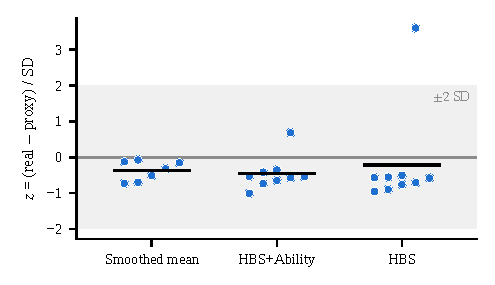
\includegraphics[width=0.6\linewidth]{figures/pair_validity.pdf}
  \caption{Real minus proxy-expected Brier ALC of each pair with label noise, in standard deviations of label noise, for the three submissions of Table~\ref{tab:proxy}. Bars mark the mean of each submission; the shaded band is $\pm 2$ standard deviations.}
  \label{fig:pairs}
\end{figure}

\paragraph{Reports that did not inform the design.} Because the reports of the smoothed mean and HBS+Ability informed the design of HBS, we repeated the comparisons of Table~\ref{tab:labelonly} with the official baseline, the smoothed mean, the ablation and the own-label predictor on the other six reports: every difference keeps its sign and changes by at most 0.0012.

\paragraph{Choice of roots.} For the 43 pairs whose budget-0 prediction is unknown, from the four early reports and the report of HBS+Ability, we chose between $r_j$ and $1 - r_j$ using the rates of the same benchmark in the reports whose prediction is known. Applied to the 26 pairs whose root is known, with references from the other known reports, this rule picks the correct root for 25 and lands within 0.1 of it for all 26; every benchmark appears in all three known reports, and the miss is a pair near 0.5, where the two roots nearly coincide. Because the rule picks the root closer to the benchmark's other rates, it can only tighten the clustering of rates by benchmark, which may explain part of the higher share on all 69 pairs than on the 26 known. Table~\ref{tab:roots} repeats the main comparisons of Table~\ref{tab:labelonly} on the 26 known pairs alone, with all 43 inferred roots flipped, and under two models of random errors, each with 40 assignments of 300 label sequences. Uniform flips flip each inferred root with probability 0.20, the upper end of the 95\% interval for the rule's error rate. Weighted flips flip each root with its probability of being wrong if rates scatter normally around the mean rate of their benchmark over the known pairs, with the standard deviation of the known pairs around these means, 0.115 (with 19 degrees of freedom). Widening it by the uncertainty of each benchmark mean, with normal or Student-$t$ tails, raises the expected number of flips from 2.1 to 2.6 or 2.8. This probability exceeds 0.1 for nine of the 43 pairs, all with rates within 0.1 of 0.5, where a flip changes the rate by at most 0.2, and the expected number of flips is 2.1. The advantages of HBS over the official baseline and the smoothed mean hold in every case, and under weighted flips every comparison keeps its sign. The advantage over HBS without benchmark pooling holds on the known pairs and with all roots flipped, but reverses in some uniform assignments. The comparison with the own-label predictor and the share of the gap due to benchmark difficulty hold on the known pairs, where the share is 56\%, but reverse when all 43 roots are flipped, which would contradict the rates of the same benchmarks in other reports, and become uncertain under uniform flips, which break the clustering of rates by benchmark that the rule relies on. The intervals of Tables~\ref{tab:labelonly} and~\ref{tab:prior} hold the inferred roots fixed. The roots of HBS+Ability are inferred before those of the four early reports, whose references include them; with references from the 26 known pairs alone, none of the 34 early roots changes.

\paragraph{Benchmark-difficulty diagnostic.} The diagnostic replaces $\mu_0$ by the benchmark's mean rate over the pairs of the other seven reports, in each of which every test benchmark appears; $\kappa_0$ and $\kappa_1$ keep their values, so labels on other benchmarks and of other subjects on the same benchmark still dilute this mean. It is estimated from 7 to 10 pairs, so part of the remaining gap is its estimation error. With $\alpha = 3$, it scores 0.162 and closes 58\% of the gap between HBS and the oracle (95\% interval 54 to 61\%); fixing $g_b$ at that mean instead ($\kappa_0 \to \infty$) closes 59\%. With $\alpha = 6$, used in Figures~\ref{fig:teaser} and~\ref{fig:gap}, it closes 65\%. On the 26 known pairs, the shares are 54\% and 56\%.

\begin{table}[ht]
  \caption{Change in Brier ALC of each alternative relative to HBS, and the share of HBS's gap to the oracle closed by knowing each benchmark's rate ($\alpha = 6$), under different choices of the 43 inferred roots. Uniform flips flip each root with probability 0.20; weighted flips use each root's estimated probability of error.}
  \label{tab:roots}
  \centering
  \small
  \begin{tabular}{lrrrrr}
    \toprule
    Roots & Baseline & Smoothed mean & No pooling & Own-label & Share \\
    \midrule
    As inferred, 69 pairs (Table~\ref{tab:labelonly}) & $+0.028$ & $+0.003$ & $+0.003$ & $+0.002$ & 0.65 \\
    26 known pairs only & $+0.024$ & $+0.005$ & $+0.005$ & $+0.003$ & 0.56 \\
    All 43 flipped & $+0.017$ & $+0.010$ & $+0.006$ & $-0.004$ & $-0.12$ \\
    Uniform flips, minimum over 40 & $+0.019$ & $+0.001$ & $-0.001$ & $-0.004$ & $-0.12$ \\
    Uniform flips, maximum over 40 & $+0.029$ & $+0.004$ & $+0.004$ & $+0.003$ & 0.53 \\
    Weighted flips, minimum over 40 & $+0.027$ & $+0.003$ & $+0.003$ & $+0.002$ & 0.62 \\
    Weighted flips, maximum over 40 & $+0.028$ & $+0.003$ & $+0.003$ & $+0.002$ & 0.65 \\
    \bottomrule
  \end{tabular}
\end{table}

\paragraph{HBS+Prior.} Table~\ref{tab:prior} gives the effect of the LLM prior on the 69 pairs. From budget 1 onward, the proxy uses the measured priors. At budget 0, it models the prior for the $k$-th evaluation item of a pair as the $K_0$-shrunk mean of $k$ ratings drawn around the benchmark's mean rating with the standard deviation of single ratings on the training benchmarks, 0.205; the mean rating is recovered by undoing the shrinkage of $\mu_b$ over the $n_b$ evaluation items of benchmark $b$ in the measurement run, summed over its pairs, and $|E_j|$ is read from each report. Each pair is simulated as if its items were rated first, which slightly understates the prior's accumulation when two pairs share a benchmark, the simulated ratings are drawn independently rather than constrained to the recovered mean, and the model ignores any correlation between an item's rating and its outcome. From budget 1, every report uses the measured $\mu_b$. Two benchmarks had two pairs in the measurement run; because an item shared by both pairs is rated once, the number of distinct rated items $|I_b|$ of Equation~\eqref{eq:prior} lies between the larger pair's $|E_j|$ and $n_b$, and over this range the recovered mean rating changes by at most 0.010. The variants with the prior from budget 0 and from budget 1 differ only at budget 0, whose weight is 0.1: its gain of 0.030 accounts for their difference of 0.003. Placing $\mu_b$ in the global rate follows the structure of HBS; fixing $g_b$ at $\mu_b$ instead ($\kappa_0 \to \infty$), so that labels on other benchmarks do not dilute it, improves the proxy score by a further 0.0006, and the final submission does so (Section~\ref{sec:prior}). Changed one at a time from the settings of HBS, the spread factor of 1.5 gains 0.0010, $\kappa_0 \to \infty$ 0.0006 and $\alpha = 4$ nothing; together they gain 0.0017. In the measurement run, $r_j$ is known from budget 0, and the budget-1 error $e = |\mu_b - r_j|$ leaves the candidates $\mu_b = r_j \pm e$, whose budget-3 predictions have ECE values $|0.1 - e|$ and $0.1 + e$; these differ whenever $e > 0$, and no prior exceeded 0.89, so $\mu_b + 0.1$ was never clipped. Equivalently, because the measurement submission predicts the constants $\mu_b$ and $\mu_b + 0.1$ within each pair at budgets 1 and 3, $\Brier_j(3) - \Brier_j(1) = 0.01 + 0.2(\mu_b - r_j)$ gives the sign directly. On the training benchmarks, whose rates lie closer to 0.35, the same procedure gained only about 0.002 in simulation, which suggests that a benchmark prior helps most when rates are extreme, as in the test pool. The improvement changes little with $K_0$, the rating order or redraws of each prior (Table~\ref{tab:prior_robust}).

\paragraph{Accuracy of the priors.} Across the seven test benchmarks, the priors order the benchmarks' mean success rates with Kendall's $\tau = 0.62$ and lower the mean absolute error from 0.22 for the constant 0.35 to 0.15, but they are compressed: regressing the priors on the mean rates gives a slope of 0.38. With the settings of HBS, the prior lowers the expected Brier ALC on five of the seven benchmarks and on 51 of the 69 pairs; removing any one benchmark leaves an improvement of 0.0057 to 0.0088, and the jackknife standard error over benchmarks, 0.0033, is larger than the interval of Table~\ref{tab:prior} suggests. With the final settings, the prior recovers 48\% of the diagnostic's gain with $\alpha = 6$ (54\% with $\alpha = 3$), improves on HBS by 0.010 on the 26 pairs with known roots, helps on five of the seven benchmarks and 54 of the 69 pairs, removing any one benchmark leaves 0.0063 to 0.0114, and redrawing the priors 20 times changes the improvement with a standard deviation of 0.0012. Table~\ref{tab:prior_robust} collects the checks of Section~\ref{sec:prior}. The priors were redrawn 20 times from their sampling distribution (the mean of $n$ ratings with standard deviation 0.205, where $n$ is the number of items rated in the measurement run); the order of the items was permuted 200 times for fixed ratings; and $K_0$, set to 5 before the measurement, was varied from 0 to 20. In the formative run of HBS+Prior with the settings of HBS (978186), predictions at budgets 1 and 3 are constant within five of the nine pairs and nearly constant within the other four, where only the corrections of Equation~\eqref{eq:corrections} vary, so both budgets approximately identify each pair's rate: Equation~\eqref{eq:identity} applied to budgets 1 and 3 gives estimates of $r_j(1 - r_j)$ that agree exactly for the five pairs and to within 0.004 for the others. Of the two roots, we take the one closer to the benchmark's mean rate over the 69 pairs. The close agreement of the two budgets also indicates that the small variation within the four pairs hardly affects Equation~\eqref{eq:identity}. In the final submission's run (1013135), the two budgets agree exactly for four pairs and to within 0.004 for the other five. In both runs, all nine pairs come from the seven test benchmarks, we use the estimate from budget 1, every chosen root lies at least 0.07 from 0.5, and the two roots differ in their distance to the benchmark's mean rate by at least 0.14. Table~\ref{tab:final_run} compares both runs with the proxy's expectations on their pairs.

\paragraph{Settings chosen leave-one-benchmark-out.} In the leave-one-report-out search of Section~\ref{sec:prior}, $K_0$ changes the result by less than 0.0001. That selection holds out draws, but every report contains the same seven benchmarks and priors. Holding out each benchmark in turn instead, and choosing from the grid of Section~\ref{sec:prior} with $K_0 = 5$ the setting that is best on the pairs of the other six (600 label sequences per report), every fold keeps $\kappa_0 \to \infty$, but the spread factor ranges from 1.25 to 2 and $\alpha$ from 3 to 6. On the held-out benchmarks, the chosen settings improve on HBS by 0.0061, against 0.0089 for the final settings fixed in advance and 0.0073 for the prior without spread; against the latter, five of the seven benchmarks gain, but the average changes by $+0.0012$. Whether spreading the prior helps on new benchmarks is therefore not established.

\begin{table}[ht]
  \caption{HBS with the LLM benchmark prior on the 69 real pairs. The priors are fixed at the values measured in Section~\ref{sec:measure}, so the 95\% intervals, from resampling whole reports, cover label noise and the sampling of pairs, but neither the sampling error of the priors (Table~\ref{tab:prior_robust}) nor benchmarks outside the test pool. A jackknife over the seven benchmarks gives a standard error of 0.0033 with the settings of HBS (approximate 95\% interval from $-0.015$ to $+0.001$) and 0.0048 with the final settings of Section~\ref{sec:prior}. Changes are computed before rounding; negative changes are improvements.}
  \label{tab:prior}
  \centering
  \small
  \begin{tabular}{lrl}
    \toprule
    Predictor & Brier ALC & Change from HBS \\
    \midrule
    HBS & 0.179 & --- \\
    HBS+Prior, prior used from budget 1 & 0.175 & $-0.0044$ $[-0.0052, -0.0035]$ \\
    HBS+Prior, prior used from budget 0 & 0.171 & $-0.0073$ $[-0.0087, -0.0059]$ \\
    HBS+Prior, final settings (final submission) & 0.170 & $-0.0090$ $[-0.0112, -0.0068]$ \\
    Each benchmark's rate known, $\alpha = 3$ (diagnostic) & 0.162 & $-0.0166$ $[-0.0185, -0.0149]$ \\
    Each benchmark's rate known, $\alpha = 6$ (diagnostic) & 0.160 & $-0.0186$ $[-0.0204, -0.0171]$ \\
    \bottomrule
  \end{tabular}
\end{table}

\begin{table}[ht]
  \caption{Change in Brier ALC of HBS+Prior with the settings of HBS (prior from budget 0) relative to HBS on the 69 pairs under different checks. Negative changes are improvements.}
  \label{tab:prior_robust}
  \centering
  \small
  \begin{tabular}{lr}
    \toprule
    Check & Change in Brier ALC \\
    \midrule
    As submitted ($K_0 = 5$), 95\% interval over reports & $-0.0073$ $[-0.0087, -0.0059]$ \\
    26 pairs with known roots & $-0.0082$ \\
    $K_0 = 0$, 2, 10, 20 & $-0.0078$, $-0.0077$, $-0.0069$, $-0.0061$ \\
    Item order permuted 200 times & $-0.0073$ (SD 0.0001) \\
    Priors redrawn 20 times & $-0.0073$ (SD 0.0008) \\
    \bottomrule
  \end{tabular}
\end{table}

\begin{table}[ht]
  \caption{The formative runs of HBS+Prior with the settings of HBS (978186) and of the final submission (1013135) against the proxy's expectations on their nine pairs each. Rates are recovered from budget 1 of each run, checked against budget 3, with the root closer to the benchmark's mean rate over the 69 pairs. The budget-0 expectation for HBS involves no labels and hence no label noise; the label-noise standard deviation of the Brier ALC is 0.007 for both runs.}
  \label{tab:final_run}
  \centering
  \small
  \begin{tabular}{lrrrrrrr}
    \toprule
    Budget & 0 & 1 & 3 & 7 & 15 & 31 & Brier ALC \\
    \midrule
    Observed, 978186 & 0.190 & 0.192 & 0.183 & 0.163 & 0.163 & 0.151 & 0.174 \\
    Expected, HBS & 0.224 & 0.201 & 0.181 & 0.167 & 0.160 & 0.156 & 0.180 \\
    Expected, HBS+Prior & 0.194 & 0.182 & 0.173 & 0.165 & 0.159 & 0.155 & 0.171 \\
    \midrule
    Observed, \finalid & 0.164 & 0.152 & 0.152 & 0.149 & 0.148 & 0.148 & 0.151 \\
    Expected, HBS & 0.217 & 0.189 & 0.168 & 0.155 & 0.147 & 0.143 & 0.168 \\
    Expected, final settings & 0.182 & 0.171 & 0.162 & 0.152 & 0.146 & 0.143 & 0.159 \\
    \bottomrule
  \end{tabular}
\end{table}

\paragraph{Baselines and tuning grids.} The official baseline predicts the mean of the pair's revealed labels, and 0.5 without labels. The own-label Bayes predictor takes as its prior the success rates $r_{j'}$ of the other 68 pairs, with equal weights, and predicts the posterior mean $\sum_{j'} r_{j'}^{k+1}(1 - r_{j'})^{t-k} / \sum_{j'} r_{j'}^{k}(1 - r_{j'})^{t-k}$ after $k$ successes in its own $t$ labels. HBS without pooling is 0.0006 worse than this predictor, so HBS beats it through pooling. The mixture prior replaces the pair prior of HBS, $\mathrm{Beta}(\alpha\pi_{sb}, \alpha(1 - \pi_{sb}))$, by a mixture with a near-unsolvable component $\mathrm{Beta}(km, k(1 - m))$ of weight $w$, and predicts the exact posterior mean, reweighting the components by their Beta-Binomial likelihoods of the pair's labels; we search $w \in \{0, 0.1, \dots, 0.4\}$, $m \in \{0.02, 0.05, 0.1\}$ and $k \in \{5, 10, 30\}$. Re-tuning searches $\mu_0 \in \{0.3, 0.35, 0.4\}$, $\alpha \in \{2, 3, 4, 6\}$ and $\kappa_1 \in \{1, 3, 6\}$. Both select leave-one-report-out.

\FloatBarrier
\section{LLM experiments}
\label{app:llm}

Tables~\ref{tab:bench} and~\ref{tab:bench_means} and Figure~\ref{fig:text}a give the anchored benchmark-level ratings of Section~\ref{sec:text} on the four held-out training benchmarks, and Figure~\ref{fig:text}b compares HBS+ItemLLM with the proxy at each budget. Most of the gain of Qwen3.8-27B on these benchmarks comes from \bench{multi\_swebench}, and its estimates are compressed toward the middle, as on the test benchmarks (Appendix~\ref{app:robust}). Four benchmarks are too few to select a model reliably; only Qwen3.8-27B was measured on the test benchmarks, and the twelve-anchor prompt of HBS+Prior could not be validated on the training benchmarks.

\paragraph{HBS+ItemLLM.} With $L$ the labeled items of the target's benchmark, from any subject, $c = (z_i + \sum_{k \in L} z_k) / (|L| + 1)$, so the shift equals $\gamma\, |L|\, (z_i - \bar z_L) / (|L| + 1)$ with $\gamma = 0.5$ at every budget, and it vanishes at budget 0. On the four multi-subject training benchmarks, the leave-one-benchmark-out probe scores, standardized as in HBS+ItemLLM (Appendix~\ref{app:repro}), lie at most 4.4 from their benchmark's mean, have a within-benchmark standard deviation of 0.59 to 1.02 and a mean within-subject correlation with the outcomes of 0.12 to 0.23. On the real draw, six of the nine pairs score worse than the proxy expects for HBS at each of budgets 1, 3 and 7, and the two subjects of one benchmark account for about 70\% of the loss; their shifts are centered on the same labeled items, the labels of both subjects on that benchmark. At budget 31, three pairs lose and one gains by more than five standard deviations of label noise.

Table~\ref{tab:itemllm} simulates the shift on the same nine pairs, with their recovered rates and evaluation sizes, against HBS on the same labels (300 label sequences). Each item receives an outcome and a synthetic score $z = \sigma(\rho u + \sqrt{1 - \rho^2}\, e)$, where $u$ is the outcome standardized within the pair and $e$ is standard normal; unless stated otherwise, the scores are independent across items. As in HBS+ItemLLM, $L$ holds the labeled items of both subjects of a benchmark, so $|L| = 2t$ at budget $t$ when two subjects share it, and the extreme score below is placed at the first revealed item of one of them. Scores like those on the training benchmarks leave HBS nearly unchanged. Uninformative scores, even for 5\% of the items or on a quarter of the benchmarks, cause losses that persist to budget 31, and so do scores that correlate negatively with the outcomes. Independent scores reproduce the average pattern only if they spread more than ten times as widely as on the training benchmarks and correlate with the outcomes at about 0.8, four times the training value; such scores push predictions toward 0 or 1, and an inaccurate $c$ moves whole pairs the wrong way until enough labels arrive. We consider this regime implausible for a probe that ranks training items with a Spearman correlation below 0.3, and an artifact of assuming the same independent scores for every item. A cause local to the benchmark that carries most of the loss fits better: with training-like scores elsewhere, a single score of 12 at its first revealed item raises the mean Brier score by 0.063 at budget 1. A score this far from the mean is almost three times the largest deviation on the training benchmarks, so this scenario only illustrates how fast such an effect fades. This effect fades faster than observed, to 0.014 at budget 3 and 0.001 at budget 7, because that item's weight in $c$ falls as $1/(|L| + 1)$; several extreme scores among the early items would fade more slowly. The aggregated feedback cannot distinguish these explanations, and none of them requires the probe to have transferred.

\begin{table}[ht]
  \caption{Change in Brier score of HBS+ItemLLM relative to HBS at budgets 1 to 31 on its draw: the real run against the proxy's expectation for HBS, and synthetic scores with spread $\sigma$ and correlation $\rho$ with the outcomes. On the training benchmarks, $\sigma$ is 0.59 to 1.02 and $\rho$ is 0.12 to 0.23. With large $\sigma$, an inaccurate $c$ at low budgets pushes all predictions of a pair toward 0 or 1.}
  \label{tab:itemllm}
  \centering
  \small
  \begin{tabular}{>{\raggedright\arraybackslash}p{0.44\linewidth}rrrrr}
    \toprule
    Item scores & 1 & 3 & 7 & 15 & 31 \\
    \midrule
    Real run & $+0.070$ & $+0.040$ & $+0.024$ & $-0.000$ & $-0.002$ \\
    $\sigma = 1$, $\rho = 0.2$ & $-0.002$ & $-0.003$ & $-0.003$ & $-0.004$ & $-0.004$ \\
    $\sigma = 1$, $\rho = 0.2$; score 12 at the first revealed item of the benchmark with most of the loss & $+0.063$ & $+0.014$ & $+0.001$ & $-0.003$ & $-0.003$ \\
    $\sigma = 3$, $\rho = 0$ & $+0.050$ & $+0.054$ & $+0.047$ & $+0.041$ & $+0.038$ \\
    $\sigma = 1$, $\rho = -0.2$ & $+0.015$ & $+0.016$ & $+0.014$ & $+0.013$ & $+0.012$ \\
    $\sigma = 3$, $\rho = -0.5$ & $+0.092$ & $+0.101$ & $+0.091$ & $+0.084$ & $+0.079$ \\
    $\sigma = 1$, $\rho = 0.2$; 5\% of items with $\sigma = 20$, $\rho = 0$ & $+0.021$ & $+0.027$ & $+0.021$ & $+0.015$ & $+0.013$ \\
    $\sigma = 6$, $\rho = 0.6$; each benchmark $\rho = 0$ with probability 0.25 & $+0.050$ & $+0.047$ & $+0.035$ & $+0.025$ & $+0.020$ \\
    $\sigma = 4$, $\rho = 0.45$ & $+0.016$ & $+0.011$ & $+0.002$ & $-0.005$ & $-0.008$ \\
    $\sigma = 8$, $\rho = 0.7$ & $+0.033$ & $+0.020$ & $+0.006$ & $-0.007$ & $-0.011$ \\
    $\sigma = 12$, $\rho = 0.8$ & $+0.050$ & $+0.031$ & $+0.012$ & $-0.002$ & $-0.008$ \\
    $\sigma = 16$, $\rho = 0.85$ & $+0.065$ & $+0.041$ & $+0.018$ & $+0.001$ & $-0.004$ \\
    \bottomrule
  \end{tabular}
\end{table}

\begin{table}[ht]
  \caption{Budget-0 priors from anchored LLM ratings on the four held-out training benchmarks. Brier is the mean over the four benchmarks of the squared error over all responses to the rated items. Kendall's $\tau$ compares the predicted and actual orderings of the benchmarks and is undefined for the single-item rows, which predict $0.35 + w(\rho_i - 0.35)$ for each item with $w \in \{0, 0.25, 0.5, 0.75, 1\}$ chosen in hindsight ($w = 0.5$) or leave-one-benchmark-out.}
  \label{tab:bench}
  \centering
  \small
  \begin{tabular}{lrr}
    \toprule
    Budget-0 prior & Kendall $\tau$ & Brier \\
    \midrule
    Constant 0.35 (HBS) & --- & 0.233 \\
    Qwen3-8B, mean rating of the benchmark & 0.33 & 0.237 \\
    Qwen3.5-9B, mean rating of the benchmark & $-0.67$ & 0.256 \\
    Qwen3-32B, mean rating of the benchmark & 0.00 & 0.285 \\
    Qwen3.8-27B, mean rating of the benchmark & 0.67 & 0.217 \\
    Qwen3.8-27B, single item, shrinkage chosen in hindsight & --- & 0.220 \\
    Qwen3.8-27B, single item, shrinkage chosen LOBO & --- & 0.231 \\
    Oracle that knows each benchmark's rate & 1.00 & 0.199 \\
    \bottomrule
  \end{tabular}
\end{table}

\begin{table}[ht]
  \caption{Mean predicted success rate of each held-out training benchmark from anchored ratings, against its actual mean rate on the rated items.}
  \label{tab:bench_means}
  \centering
  \small
  \begin{tabular}{lrrrr}
    \toprule
    & \bench{multi\_swebench} & \bench{researchcodebench} & \bench{real\_webagents} & \bench{matharena} \\
    \midrule
    Actual & 0.125 & 0.341 & 0.366 & 0.645 \\
    Qwen3-8B & 0.206 & 0.108 & 0.378 & 0.340 \\
    Qwen3.5-9B & 0.535 & 0.532 & 0.459 & 0.514 \\
    Qwen3-32B & 0.330 & 0.384 & 0.700 & 0.210 \\
    Qwen3.8-27B & 0.202 & 0.359 & 0.407 & 0.394 \\
    \bottomrule
  \end{tabular}
\end{table}

\begin{figure}[ht]
  \centering
  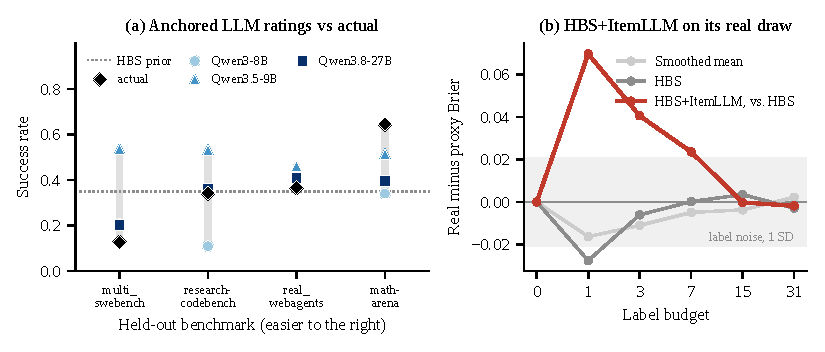
\includegraphics[width=\linewidth]{figures/text_difficulty.pdf}
  \caption{(a) Mean success rate predicted by anchored prompts for each held-out training benchmark (markers) against the actual rate (diamonds); dotted line: the budget-0 prediction of HBS. (b) Real minus proxy-expected Brier score per budget on each submission's own draw; HBS+ItemLLM is compared with the expectation for HBS.}
  \label{fig:text}
\end{figure}

\clearpage
\section*{NeurIPS Paper Checklist}



\begin{enumerate}

\item {\bf Claims}
    \item[] Question: Do the main claims made in the abstract and introduction accurately reflect the paper's contributions and scope?
    \item[] Answer: \answerYes{}
    \item[] Justification: The abstract and the introduction (Section~\ref{sec:intro}) state three contributions, supported in Sections~\ref{sec:proxy} and~\ref{sec:experiments} (Proposition~\ref{prop:identity}, Tables~\ref{tab:proxy}, \ref{tab:labelonly} and~\ref{tab:prior}, Figures~\ref{fig:draws} and~\ref{fig:gap}); their scope (one competition, 69 pairs, four training benchmarks) is stated in Section~\ref{sec:discussion}.
    \item[] Guidelines:
    \begin{itemize}
        \item The answer \answerNA{} means that the abstract and introduction do not include the claims made in the paper.
        \item The abstract and/or introduction should clearly state the claims made, including the contributions made in the paper and important assumptions and limitations. A \answerNo{} or \answerNA{} answer to this question will not be perceived well by the reviewers. 
        \item The claims made should match theoretical and experimental results, and reflect how much the results can be expected to generalize to other settings. 
        \item It is fine to include aspirational goals as motivation as long as it is clear that these goals are not attained by the paper. 
    \end{itemize}

\item {\bf Limitations}
    \item[] Question: Does the paper discuss the limitations of the work performed by the authors?
    \item[] Answer: \answerYes{}
    \item[] Justification: Section~\ref{sec:discussion} (Limitations) covers the proxy's assumptions and pessimism, the inferred roots, the number of pairs and benchmarks, the single real draw for the item-level LLM shift, the single measurement of the LLM prior, and the model sizes we tested.
    \item[] Guidelines:
    \begin{itemize}
        \item The answer \answerNA{} means that the paper has no limitation while the answer \answerNo{} means that the paper has limitations, but those are not discussed in the paper. 
        \item The authors are encouraged to create a separate ``Limitations'' section in their paper.
        \item The paper should point out any strong assumptions and how robust the results are to violations of these assumptions (e.g., independence assumptions, noiseless settings, model well-specification, asymptotic approximations only holding locally). The authors should reflect on how these assumptions might be violated in practice and what the implications would be.
        \item The authors should reflect on the scope of the claims made, e.g., if the approach was only tested on a few datasets or with a few runs. In general, empirical results often depend on implicit assumptions, which should be articulated.
        \item The authors should reflect on the factors that influence the performance of the approach. For example, a facial recognition algorithm may perform poorly when image resolution is low or images are taken in low lighting. Or a speech-to-text system might not be used reliably to provide closed captions for online lectures because it fails to handle technical jargon.
        \item The authors should discuss the computational efficiency of the proposed algorithms and how they scale with dataset size.
        \item If applicable, the authors should discuss possible limitations of their approach to address problems of privacy and fairness.
        \item While the authors might fear that complete honesty about limitations might be used by reviewers as grounds for rejection, a worse outcome might be that reviewers discover limitations that aren't acknowledged in the paper. The authors should use their best judgment and recognize that individual actions in favor of transparency play an important role in developing norms that preserve the integrity of the community. Reviewers will be specifically instructed to not penalize honesty concerning limitations.
    \end{itemize}

\item {\bf Theory assumptions and proofs}
    \item[] Question: For each theoretical result, does the paper provide the full set of assumptions and a complete (and correct) proof?
    \item[] Answer: \answerYes{}
    \item[] Justification: Proposition~\ref{prop:identity} states its assumption (a constant budget-0 prediction within the pair) and is followed by a complete proof (Section~\ref{sec:proxy}).
    \item[] Guidelines:
    \begin{itemize}
        \item The answer \answerNA{} means that the paper does not include theoretical results. 
        \item All the theorems, formulas, and proofs in the paper should be numbered and cross-referenced.
        \item All assumptions should be clearly stated or referenced in the statement of any theorems.
        \item The proofs can either appear in the main paper or the supplemental material, but if they appear in the supplemental material, the authors are encouraged to provide a short proof sketch to provide intuition. 
        \item Inversely, any informal proof provided in the core of the paper should be complemented by formal proofs provided in appendix or supplemental material.
        \item Theorems and Lemmas that the proof relies upon should be properly referenced. 
    \end{itemize}

    \item {\bf Experimental result reproducibility}
    \item[] Question: Does the paper fully disclose all the information needed to reproduce the main experimental results of the paper to the extent that it affects the main claims and/or conclusions of the paper (regardless of whether the code and data are provided or not)?
    \item[] Answer: \answerYes{}
    \item[] Justification: Section~\ref{sec:method} and Table~\ref{tab:hparams} fully specify HBS and HBS+Prior; Sections~\ref{sec:setup}, \ref{sec:proxy} and~\ref{sec:text} and Appendices~\ref{app:prompts} and~\ref{app:repro} give the simulator, the proxy, the measurement submission, prompts and data; the repository README gives the exact commands. Reproducing the proxy and the measurement analysis requires a team's own formative logs, which the competition keeps private.
    \item[] Guidelines:
    \begin{itemize}
        \item The answer \answerNA{} means that the paper does not include experiments.
        \item If the paper includes experiments, a \answerNo{} answer to this question will not be perceived well by the reviewers: Making the paper reproducible is important, regardless of whether the code and data are provided or not.
        \item If the contribution is a dataset and\slash or model, the authors should describe the steps taken to make their results reproducible or verifiable. 
        \item Depending on the contribution, reproducibility can be accomplished in various ways. For example, if the contribution is a novel architecture, describing the architecture fully might suffice, or if the contribution is a specific model and empirical evaluation, it may be necessary to either make it possible for others to replicate the model with the same dataset, or provide access to the model. In general. releasing code and data is often one good way to accomplish this, but reproducibility can also be provided via detailed instructions for how to replicate the results, access to a hosted model (e.g., in the case of a large language model), releasing of a model checkpoint, or other means that are appropriate to the research performed.
        \item While NeurIPS does not require releasing code, the conference does require all submissions to provide some reasonable avenue for reproducibility, which may depend on the nature of the contribution. For example
        \begin{enumerate}
            \item If the contribution is primarily a new algorithm, the paper should make it clear how to reproduce that algorithm.
            \item If the contribution is primarily a new model architecture, the paper should describe the architecture clearly and fully.
            \item If the contribution is a new model (e.g., a large language model), then there should either be a way to access this model for reproducing the results or a way to reproduce the model (e.g., with an open-source dataset or instructions for how to construct the dataset).
            \item We recognize that reproducibility may be tricky in some cases, in which case authors are welcome to describe the particular way they provide for reproducibility. In the case of closed-source models, it may be that access to the model is limited in some way (e.g., to registered users), but it should be possible for other researchers to have some path to reproducing or verifying the results.
        \end{enumerate}
    \end{itemize}


\item {\bf Open access to data and code}
    \item[] Question: Does the paper provide open access to the data and code, with sufficient instructions to faithfully reproduce the main experimental results, as described in supplemental material?
    \item[] Answer: \answerYes{}
    \item[] Justification: Code and instructions are released at \url{https://github.com/kay0601/how-far-can-labels-go} (Appendix~\ref{app:repro}), and the training data are public (measurement-db, revision bc8204d). Our formative logs are private under the competition rules and are not released; the proxy scripts read a team's own logs.
    \item[] Guidelines:
    \begin{itemize}
        \item The answer \answerNA{} means that paper does not include experiments requiring code.
        \item Please see the NeurIPS code and data submission guidelines (\url{https://neurips.cc/public/guides/CodeSubmissionPolicy}) for more details.
        \item While we encourage the release of code and data, we understand that this might not be possible, so \answerNo{} is an acceptable answer. Papers cannot be rejected simply for not including code, unless this is central to the contribution (e.g., for a new open-source benchmark).
        \item The instructions should contain the exact command and environment needed to run to reproduce the results. See the NeurIPS code and data submission guidelines (\url{https://neurips.cc/public/guides/CodeSubmissionPolicy}) for more details.
        \item The authors should provide instructions on data access and preparation, including how to access the raw data, preprocessed data, intermediate data, and generated data, etc.
        \item The authors should provide scripts to reproduce all experimental results for the new proposed method and baselines. If only a subset of experiments are reproducible, they should state which ones are omitted from the script and why.
        \item At submission time, to preserve anonymity, the authors should release anonymized versions (if applicable).
        \item Providing as much information as possible in supplemental material (appended to the paper) is recommended, but including URLs to data and code is permitted.
    \end{itemize}


\item {\bf Experimental setting/details}
    \item[] Question: Does the paper specify all the training and test details (e.g., data splits, hyperparameters, how they were chosen, type of optimizer) necessary to understand the results?
    \item[] Answer: \answerYes{}
    \item[] Justification: Section~\ref{sec:method} gives all hyperparameters and how they were set; Sections~\ref{sec:setup} and~\ref{sec:proxy} give the simulator and proxy protocols and the held-out selection; Section~\ref{sec:text} and Appendix~\ref{app:prompts} give the LLM settings.
    \item[] Guidelines:
    \begin{itemize}
        \item The answer \answerNA{} means that the paper does not include experiments.
        \item The experimental setting should be presented in the core of the paper to a level of detail that is necessary to appreciate the results and make sense of them.
        \item The full details can be provided either with the code, in appendix, or as supplemental material.
    \end{itemize}

\item {\bf Experiment statistical significance}
    \item[] Question: Does the paper report error bars suitably and correctly defined or other appropriate information about the statistical significance of the experiments?
    \item[] Answer: \answerYes{}
    \item[] Justification: Table~\ref{tab:proxy} reports label-noise standard deviations and $z$-scores; Tables~\ref{tab:labelonly} and~\ref{tab:prior} report 95\% intervals from resampling whole reports, and Table~\ref{tab:labelonly} a simulator standard error; Appendix~\ref{app:robust} reports further robustness checks.
    \item[] Guidelines:
    \begin{itemize}
        \item The answer \answerNA{} means that the paper does not include experiments.
        \item The authors should answer \answerYes{} if the results are accompanied by error bars, confidence intervals, or statistical significance tests, at least for the experiments that support the main claims of the paper.
        \item The factors of variability that the error bars are capturing should be clearly stated (for example, train/test split, initialization, random drawing of some parameter, or overall run with given experimental conditions).
        \item The method for calculating the error bars should be explained (closed form formula, call to a library function, bootstrap, etc.)
        \item The assumptions made should be given (e.g., Normally distributed errors).
        \item It should be clear whether the error bar is the standard deviation or the standard error of the mean.
        \item It is OK to report 1-sigma error bars, but one should state it. The authors should preferably report a 2-sigma error bar than state that they have a 96\% CI, if the hypothesis of Normality of errors is not verified.
        \item For asymmetric distributions, the authors should be careful not to show in tables or figures symmetric error bars that would yield results that are out of range (e.g., negative error rates).
        \item If error bars are reported in tables or plots, the authors should explain in the text how they were calculated and reference the corresponding figures or tables in the text.
    \end{itemize}

\item {\bf Experiments compute resources}
    \item[] Question: For each experiment, does the paper provide sufficient information on the computer resources (type of compute workers, memory, time of execution) needed to reproduce the experiments?
    \item[] Answer: \answerYes{}
    \item[] Justification: Appendix~\ref{app:repro} lists the hardware (a CPU for HBS and the simulator; a single RTX 3090 for the LLM experiments and HBS+Prior), the run time of each experiment and the software versions.
    \item[] Guidelines:
    \begin{itemize}
        \item The answer \answerNA{} means that the paper does not include experiments.
        \item The paper should indicate the type of compute workers CPU or GPU, internal cluster, or cloud provider, including relevant memory and storage.
        \item The paper should provide the amount of compute required for each of the individual experimental runs as well as estimate the total compute. 
        \item The paper should disclose whether the full research project required more compute than the experiments reported in the paper (e.g., preliminary or failed experiments that didn't make it into the paper). 
    \end{itemize}
    
\item {\bf Code of ethics}
    \item[] Question: Does the research conducted in the paper conform, in every respect, with the NeurIPS Code of Ethics \url{https://neurips.cc/public/EthicsGuidelines}?
    \item[] Answer: \answerYes{}
    \item[] Justification: The work uses public benchmark data and our own formative feedback as permitted by the competition rules, involves no human subjects, and releases no recovered test data (Section~\ref{sec:measure}).
    \item[] Guidelines:
    \begin{itemize}
        \item The answer \answerNA{} means that the authors have not reviewed the NeurIPS Code of Ethics.
        \item If the authors answer \answerNo, they should explain the special circumstances that require a deviation from the Code of Ethics.
        \item The authors should make sure to preserve anonymity (e.g., if there is a special consideration due to laws or regulations in their jurisdiction).
    \end{itemize}


\item {\bf Broader impacts}
    \item[] Question: Does the paper discuss both potential positive societal impacts and negative societal impacts of the work performed?
    \item[] Answer: \answerYes{}
    \item[] Justification: Appendix~\ref{app:disclosure} discusses the positive impact (cheaper evaluation) and the negative impact (predicted scores trusted in place of measured ones).
    \item[] Guidelines:
    \begin{itemize}
        \item The answer \answerNA{} means that there is no societal impact of the work performed.
        \item If the authors answer \answerNA{} or \answerNo, they should explain why their work has no societal impact or why the paper does not address societal impact.
        \item Examples of negative societal impacts include potential malicious or unintended uses (e.g., disinformation, generating fake profiles, surveillance), fairness considerations (e.g., deployment of technologies that could make decisions that unfairly impact specific groups), privacy considerations, and security considerations.
        \item The conference expects that many papers will be foundational research and not tied to particular applications, let alone deployments. However, if there is a direct path to any negative applications, the authors should point it out. For example, it is legitimate to point out that an improvement in the quality of generative models could be used to generate Deepfakes for disinformation. On the other hand, it is not needed to point out that a generic algorithm for optimizing neural networks could enable people to train models that generate Deepfakes faster.
        \item The authors should consider possible harms that could arise when the technology is being used as intended and functioning correctly, harms that could arise when the technology is being used as intended but gives incorrect results, and harms following from (intentional or unintentional) misuse of the technology.
        \item If there are negative societal impacts, the authors could also discuss possible mitigation strategies (e.g., gated release of models, providing defenses in addition to attacks, mechanisms for monitoring misuse, mechanisms to monitor how a system learns from feedback over time, improving the efficiency and accessibility of ML).
    \end{itemize}
    
\item {\bf Safeguards}
    \item[] Question: Does the paper describe safeguards that have been put in place for responsible release of data or models that have a high risk for misuse (e.g., pre-trained language models, image generators, or scraped datasets)?
    \item[] Answer: \answerNA{}
    \item[] Justification: We release no data or models with a high risk of misuse; the released code predicts success rates from labels.
    \item[] Guidelines:
    \begin{itemize}
        \item The answer \answerNA{} means that the paper poses no such risks.
        \item Released models that have a high risk for misuse or dual-use should be released with necessary safeguards to allow for controlled use of the model, for example by requiring that users adhere to usage guidelines or restrictions to access the model or implementing safety filters. 
        \item Datasets that have been scraped from the Internet could pose safety risks. The authors should describe how they avoided releasing unsafe images.
        \item We recognize that providing effective safeguards is challenging, and many papers do not require this, but we encourage authors to take this into account and make a best faith effort.
    \end{itemize}

\item {\bf Licenses for existing assets}
    \item[] Question: Are the creators or original owners of assets (e.g., code, data, models), used in the paper, properly credited and are the license and terms of use explicitly mentioned and properly respected?
    \item[] Answer: \answerYes{}
    \item[] Justification: measurement-db (CC BY-SA 4.0, gated), the Qwen models (Apache 2.0) and bge-small-en-v1.5 (MIT) are cited, and their licenses are stated in Appendix~\ref{app:disclosure}; we do not redistribute the data.
    \item[] Guidelines:
    \begin{itemize}
        \item The answer \answerNA{} means that the paper does not use existing assets.
        \item The authors should cite the original paper that produced the code package or dataset.
        \item The authors should state which version of the asset is used and, if possible, include a URL.
        \item The name of the license (e.g., CC-BY 4.0) should be included for each asset.
        \item For scraped data from a particular source (e.g., website), the copyright and terms of service of that source should be provided.
        \item If assets are released, the license, copyright information, and terms of use in the package should be provided. For popular datasets, \url{paperswithcode.com/datasets} has curated licenses for some datasets. Their licensing guide can help determine the license of a dataset.
        \item For existing datasets that are re-packaged, both the original license and the license of the derived asset (if it has changed) should be provided.
        \item If this information is not available online, the authors are encouraged to reach out to the asset's creators.
    \end{itemize}

\item {\bf New assets}
    \item[] Question: Are new assets introduced in the paper well documented and is the documentation provided alongside the assets?
    \item[] Answer: \answerYes{}
    \item[] Justification: The released code is documented by a README that maps every table and figure to the command that produces it (Appendix~\ref{app:repro}), and is released under the MIT License.
    \item[] Guidelines:
    \begin{itemize}
        \item The answer \answerNA{} means that the paper does not release new assets.
        \item Researchers should communicate the details of the dataset\slash code\slash model as part of their submissions via structured templates. This includes details about training, license, limitations, etc. 
        \item The paper should discuss whether and how consent was obtained from people whose asset is used.
        \item At submission time, remember to anonymize your assets (if applicable). You can either create an anonymized URL or include an anonymized zip file.
    \end{itemize}

\item {\bf Crowdsourcing and research with human subjects}
    \item[] Question: For crowdsourcing experiments and research with human subjects, does the paper include the full text of instructions given to participants and screenshots, if applicable, as well as details about compensation (if any)? 
    \item[] Answer: \answerNA{}
    \item[] Justification: The work involves no crowdsourcing or research with human subjects.
    \item[] Guidelines:
    \begin{itemize}
        \item The answer \answerNA{} means that the paper does not involve crowdsourcing nor research with human subjects.
        \item Including this information in the supplemental material is fine, but if the main contribution of the paper involves human subjects, then as much detail as possible should be included in the main paper. 
        \item According to the NeurIPS Code of Ethics, workers involved in data collection, curation, or other labor should be paid at least the minimum wage in the country of the data collector. 
    \end{itemize}

\item {\bf Institutional review board (IRB) approvals or equivalent for research with human subjects}
    \item[] Question: Does the paper describe potential risks incurred by study participants, whether such risks were disclosed to the subjects, and whether Institutional Review Board (IRB) approvals (or an equivalent approval/review based on the requirements of your country or institution) were obtained?
    \item[] Answer: \answerNA{}
    \item[] Justification: The work involves no human subjects.
    \item[] Guidelines:
    \begin{itemize}
        \item The answer \answerNA{} means that the paper does not involve crowdsourcing nor research with human subjects.
        \item Depending on the country in which research is conducted, IRB approval (or equivalent) may be required for any human subjects research. If you obtained IRB approval, you should clearly state this in the paper. 
        \item We recognize that the procedures for this may vary significantly between institutions and locations, and we expect authors to adhere to the NeurIPS Code of Ethics and the guidelines for their institution. 
        \item For initial submissions, do not include any information that would break anonymity (if applicable), such as the institution conducting the review.
    \end{itemize}

\item {\bf Declaration of LLM usage}
    \item[] Question: Does the paper describe the usage of LLMs if it is an important, original, or non-standard component of the core methods in this research? Note that if the LLM is used only for writing, editing, or formatting purposes and does \emph{not} impact the core methodology, scientific rigor, or originality of the research, declaration is not required.
    %this research? 
    \item[] Answer: \answerYes{}
    \item[] Justification: An LLM (Qwen3.8-27B) is a component of the final submission, HBS+Prior: Section~\ref{sec:method} and Appendix~\ref{app:prompts} describe the model, prompt and settings, and Sections~\ref{sec:text} and~\ref{sec:prior} evaluate it and the other LLMs we tested. The use of a coding assistant is disclosed in Appendix~\ref{app:disclosure}.
    \item[] Guidelines:
    \begin{itemize}
        \item The answer \answerNA{} means that the core method development in this research does not involve LLMs as any important, original, or non-standard components.
        \item Please refer to our LLM policy in the NeurIPS handbook for what should or should not be described.
    \end{itemize}

\end{enumerate}

\end{document}
